\documentclass[a4paper]{article}


\usepackage[paperwidth=6in, paperheight=13in]{geometry}
\geometry{letterpaper}


\usepackage[english]{babel}
\usepackage[utf8]{inputenc}
\usepackage{amsmath}
\usepackage{graphicx}
\usepackage[colorinlistoftodos]{todonotes}
\newcommand*\circled[1]{\tikz[baseline=(char.base)]{
		\node[shape=circle,draw,inner sep=2pt] (char) {#1};}}
%\title{Model-based Development for Safe Closed-loop Medical Devices}
\title{From Verified Models to Verified Code\\ for Safe Medical Devices}
\author{Zhihao Jiang}

% \date{\today}

\begin{document}
\maketitle

% \begin{abstract}
% Your abstract.
% \end{abstract}

\section*{Thesis Problem}
Closed-loop medical devices like implantable pacemakers diagnose conditions of the patient and autonomously deliver corresponding therapies.
The fundamental challenge for developing safe closed-loop medical devices are: 
1) how to make correct diagnosis with \textbf{limited observability} on the patients' physiology? 
2) how to ensure the closed-loop interactions between \textbf{complex physiology} and device therapies are always safe?
3) how to develop devices that are general enough to safely operate on large groups of patients with \textbf{large variability} in their physiology?
%have both therapeutic and diagnostic capabilities, which are performed by increasingly sophisticated software component. 
In order to address these challenges, the safety and efficacy of closed-loop medical devices have to be evaluated within their physiological contexts, which is currently performed as clinical trials on real patients.
However, clinical trials pose significant risks to the patients involved, and safety issues found at this stage are costly to fix. 
There is urgent need to be able to evaluate device safety earlier during the development process.
%There is no transition between the engineering realm and 
%There is urgent need to identify potential safety violations earlier during the software design process.

\section*{Thesis Statement}
In this thesis, I proposed model-based approaches to evaluate the safety and efficacy of closed-loop medical devices during their development process, with implantable cardiac devices as case study.
I focused on addressing the following questions:
\begin{itemize}
	\item What can be the substitutes for real patients in closed-loop evaluations of implantable cardiac devices?
\end{itemize}
A heart model structure has been developed to model the timing of generation and conduction of electrical events in the heart.
The model structure can be configured to represent a large variety of heart conditions.
The model structure is available in both software and hardware, and is capable of generating realistic physiological signals to the devices and respond to device outputs.
%The model structure is based on clinical Electrophysiology which is also the basis for implantable cardiac devices.
%The heart model structure is abstract enough to be used during model checking, and expressive enough to represent a large variety of heart conditions.
\begin{itemize}
\item How to ensure the design of the device is safe early in the design process? 
\end{itemize}
Abstract model of the device design can be evaluated in closed-loop with models of patient physiology using model checking.
The variability of the patient is captured using non-determinism and the heart models are abstracted to capture the electrical behaviors observable to the devices.
An abstraction tree structure has been developed to balance the coverage and expressiveness of the heart models for different safety properties.
The result of closed-loop model checking provides safety and efficacy guarantee to the device design, which can contribute to the risk analysis of the device.
\begin{itemize}
	\item How to ensure the properties verified in device model still hold in device implementation?
\end{itemize}
The device model verified in model checker UPPAAL can be automatically translated into Stateflow model through a rigorous model translation tool we developed.
The Stateflow model of the device can then be generated into C code using Simulink Coder.
This toolchain enables developing the device function with a verifiable model and maintain all verified properties in the final implementation.
\begin{itemize}
	\item Can model-based approaches help before the device goes for clinical trials?
\end{itemize}
A clinical trial is only useful if its result shows statistical significance.
A failed trial is a huge cost in time and money, and poses significant risks on the patients involved.
Therefore clinical trials need to be planned carefully, with correct estimation of the size of the patient population.
In this thesis, I proposed  \emph{model-based clinical trial}, in which I use the heart model structure to construct a virtual patient population with different heart conditions.
The population captures the variability of patients' physiological conditions.
The device can then be evaluated on the virtual population, and various analysis can be performed which can provide useful insights for planning a clinical trial.

The aforementioned model-based approaches form a model-based framework for developing cyber-physical systems, which bridges the gap between the cyber domain and the physical domain.
%Model-based closed-loop evaluation can be performed%Model-based techniques can be used throughout the software design process of closed-loop medical devices, and device model can be rigorously translated into implementation. 
%\begin{itemize}
%\item How to use models to capture the variability and complexity of patient physiology while taking into account the interaction between the device and the patient?
%\end{itemize}
%Models of the physiological context can be created to represent the patients,
%\begin{itemize}
%\item What are the model-based techniques that can be applied?
%\end{itemize}
%By applying model-based techniques including model abstraction, model checking, model translation, closed-loop validation of the device software can be performed during different steps of the software design process.
%\begin{itemize}
%\item How can the results of these model-based techniques contribute to the safety and efficacy of the devices?
%\end{itemize}
%The results of these closed-loop validation provide safety and efficacy evidence of the device software, which are also compatible with the current regulation framework. 
%Applying the proposed model-based techniques can potentially reduce the time and money cost during the software development for all parties involved, including device manufacturers, the regulation agency and also the physicians.


\newpage
\section{Motivation}
Medical devices play an essential role in the care of patients around the world, and can have a life-saving effect.
To cite one example, 
%an estimated 3 million people worldwide have implanted pacemakers (a heart rhythm adjustment device), with \~600,000 added annually.
%Cardiac Pacemakers From the Patient's Perspective circ.ahajournals.org/content/105/18/2136.full
in the US, $\sim$800,000 people have an implanted defibrillator (a heart rhythm management device), with 10,000 added monthly.
%http://asktheicd.com/tile/106/english-implantable-cardioverter-defibrillator-icd/how-many-people-have-icds/
Clinical trials have presented evidence that patients implanted with defibrillators have a mortality rate reduced by up to 31\%.
% MADIT II trial
%Financially, the medical device market is worth \$289 billion.
%Of that, \$110 billion is in the US alone, with this number projected to reach \$133 billion in 2016.
%http://selectusa.commerce.gov/industry-snapshots/medical-device-industry-united-states
Examples include everything from adhesive bandages to drug infusion pumps, surgical robots, deep brain stimulation systems and devices still undergoing basic research like the artificial pancreas.
%In fact, many device companies are in the no-revenue startup phase, indicating a vigorous research environment.
These are safety-critical technologies combining hardware and software, each of which must be rigorously validated to be efficacious and safe.
\begin{figure}[t]
	\centering
	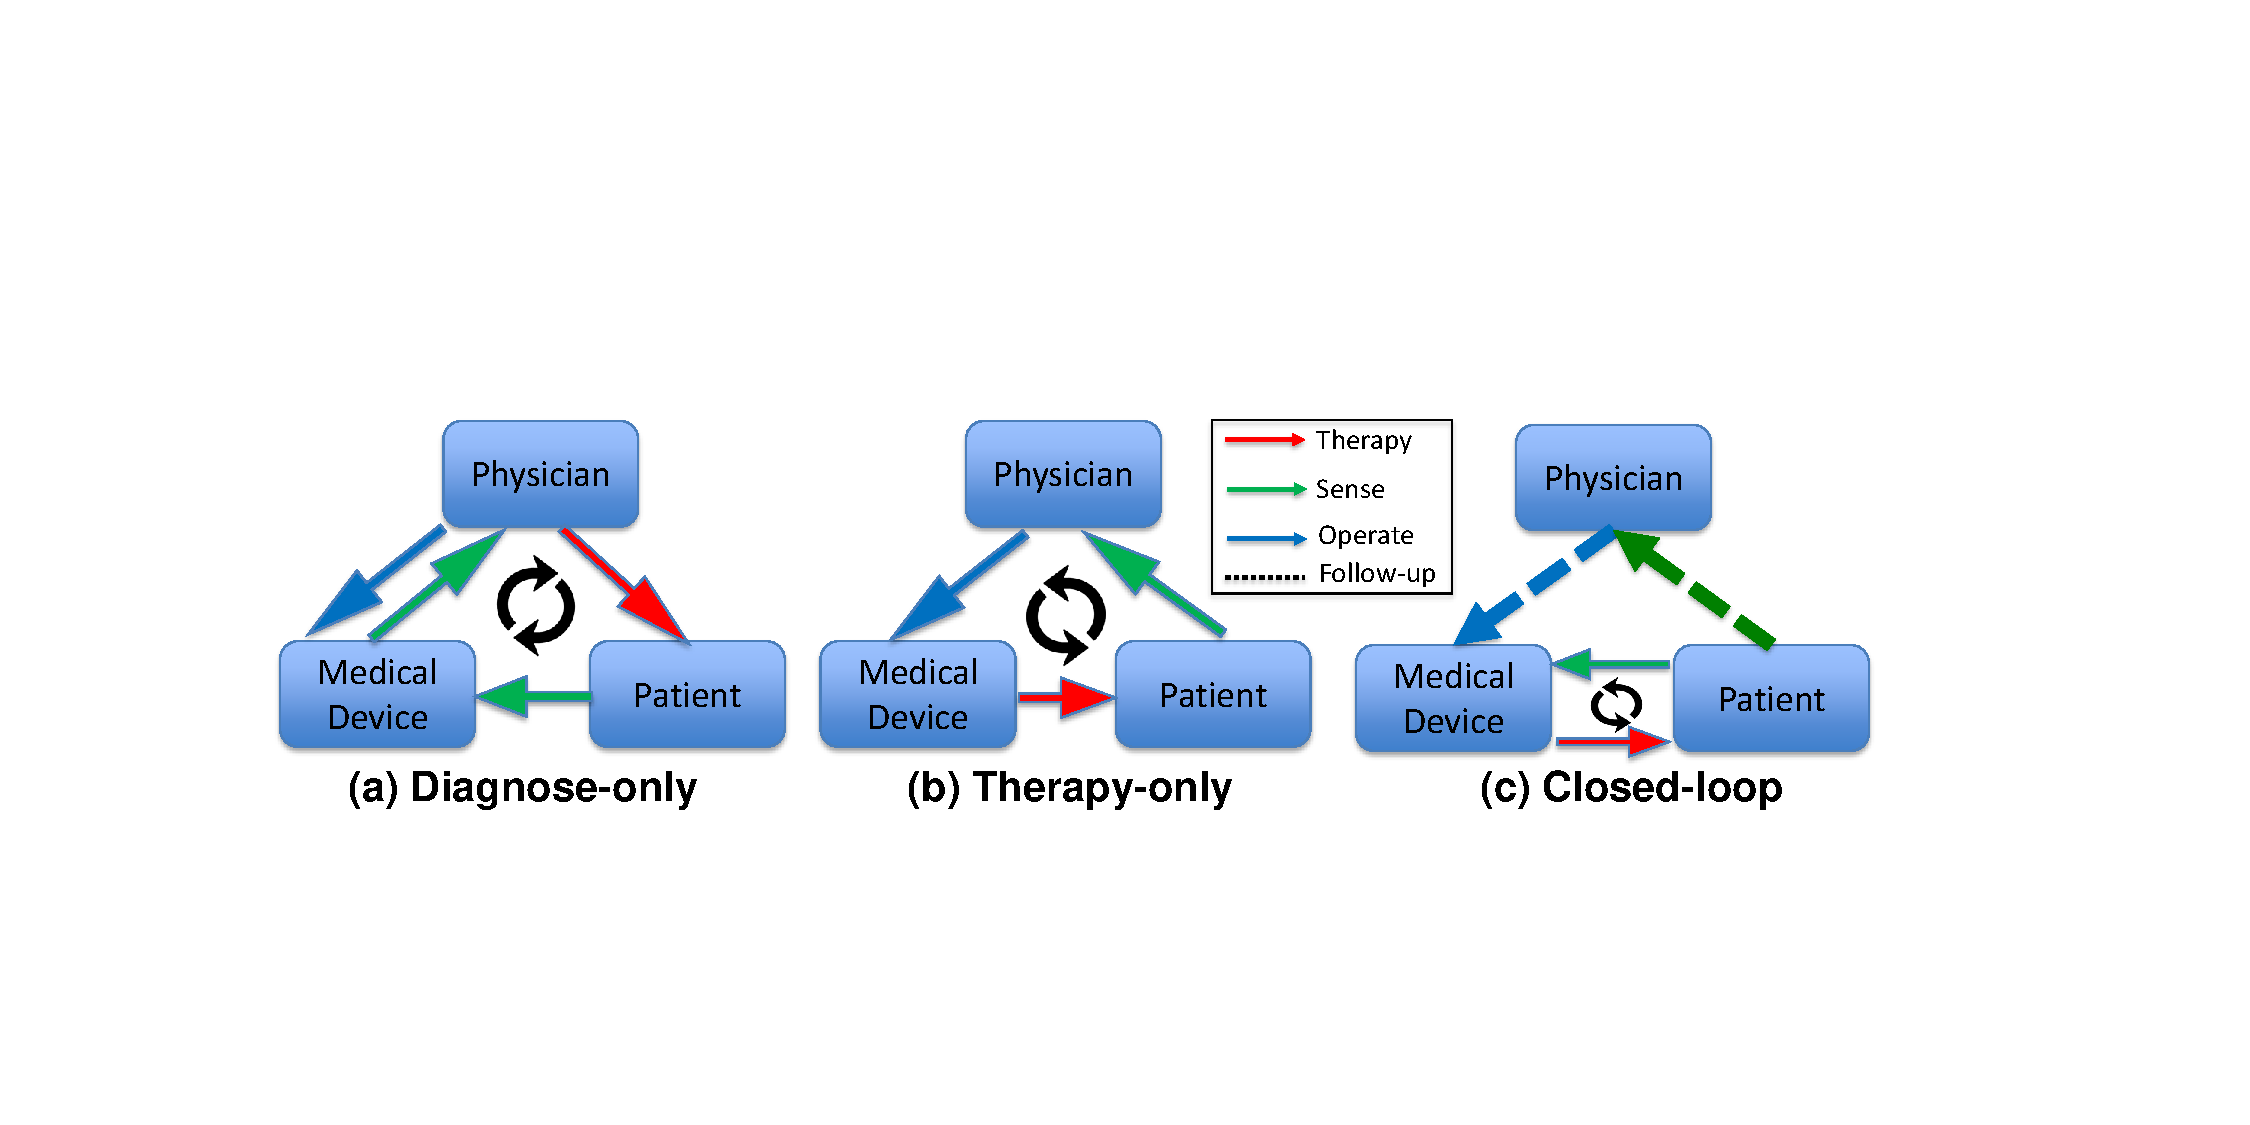
\includegraphics[scale=0.35]{figs/closed-loop.pdf}
	\caption{\small Open-loop and closed-loop medical devices. The open-loop devices has medical professionals in the loop while the closed-loop medical devices interact with patient physiology directly.}
	\label{fig:closed-loop}
\end{figure}

There are two categories of medical devices. 
One category is \emph{open-loop medical device} which has only therapeutic or diagnostic capability, i.e. infusion pumps. 
Open-loop medical devices are normally operated by professional medical care providers, which provides reliable safety guarantees (Fig. \ref{fig:closed-loop}).
On the other hand, there is an emerging category referred to as \emph{closed-loop medical devices}, which has both therapeutic and diagnostic capability.
An example of closed-loop medical devices is implantable pacemaker which diagnoses patient condition through sensed electrogram signals and deliver electrical pacing to maintain appropriate heart rhythm (Fig. \ref{fig:pacemaker}). 
Closed-loop medical devices interact with human physiology directly, and often times without human intervention.
Therefore device failures like inappropriate therapies may result in serious injuries or death of the patient.
As the result, closed-loop medical devices are categorized by the regulation agencies as the highest risk devices.
\begin{figure}[b]
	\centering
	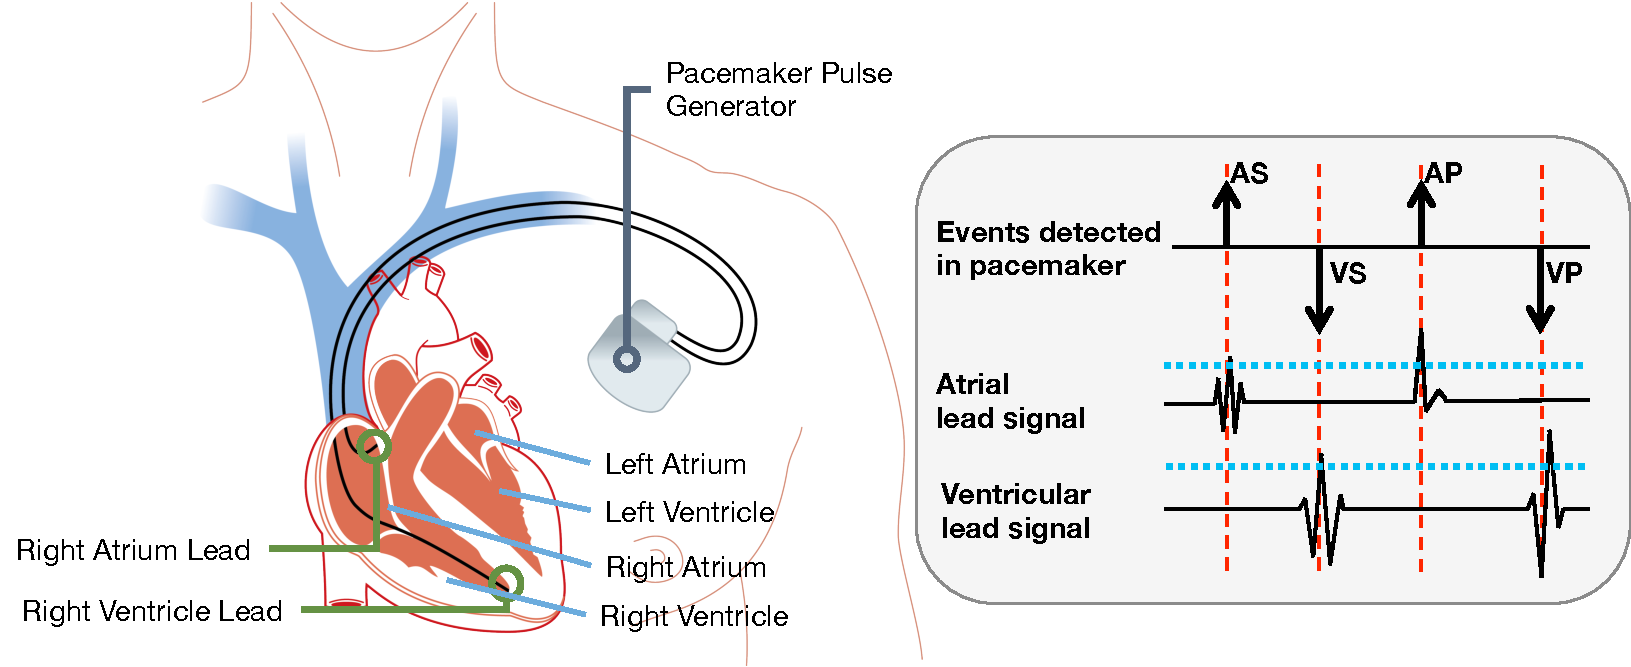
\includegraphics[scale=0.35]{figs/fig1pacemaker.pdf}
	\caption{\small Pacemaker operating in a closed-loop with the heart. The leads sense cardiac electrophysiological activity from inside the heart tissue (AS/VS = Atrial/Ventricular Sense event) and actuate the heart (AP/VP = Atrial/Ventricular Pacing event to maintain a desired heart rate.}
	\label{fig:pacemaker}
\end{figure}
%\section{Challenges for Developing Safe Closed-loop Medical Devices}
%\subsection{Sophisticated and Unreliable Software}
%To guarantee safe operation, closed-loop medical devices need to correctly identify the condition of the patient and deliver appropriate therapy.
%The complex run-time diagnoses needed for closed loop performance, and the intricate therapy delivered, has driven most diagnosis and therapy functions into software.
%As the algorithms become more sophisticated, more safety issues are related to software design. 
%According to the US Food and Drug Administration, in 1996, 10\% of all medical device recalls were caused by software-related issues. 
%This percentage rose to an average of 15\% of recalls from 2008 to 2012. 
%Implanted cardiac pacemakers and defibrillators have approximately 80,000-100,000 lines of software code which essentially makes all sensing, control and actuation decisions autonomously within the human body, over the 5-7 year device lifetime. 
%The primary challenge of high-confidence medical device software is to guarantee the device will never drive the patient into an unsafe condition even though we do not have complete understanding of the physiological plant.  
%\subsection{Closed-loop Interaction with Human Physiology}
%Closed-loop medical devices directly measure physiological signals from the patient and deliver therapy based on the diagnosis.
%The patient physiology responds to the device output and generates corresponding physiological signals to the device, therefore the safety and efficacy of the devices have to be validated within its physiological context.
%% However, the understanding of human physiology
%% Due to the knowledge gap between the domain experts and the software developers, it is impossible to encode 
%Currently the only closed-loop validation method is \emph{clinical trials}, in which the performance of the devices are evaluated on real patients.
%Clinical trials are costly in terms of time and money, while exposing enrolled patients with risky unproven therapies.
%Problems found at this late stage are also very costly to fix.
%
%
%\subsection{Model-based Design}
%\emph{Model-based Design (MBD)} can potentially enable closed-loop validation at earlier design phrase, which can potentially save development cost.
%MBD has been widely applied in industries like automotive and aviation. 
%However, MBD has not been very appealing for developing closed-loop medical devices.
%%, the device (or a model thereof) is connected to a \emph{model} of the ``physiological plant" it interacts with.
%%By high confidence verification, researchers mean that under all possible behaviors of the physiological models, the device will act correctly.
%The major challenge is the lack of appropriate physiological models that interact with the device model.
%There are two major differences between modeling physiology and modeling man-made systems:
%first, physiology is much more complex and less well-understood than man-made systems like cars and airplanes, and spans several scales from the molecular to the entire human body.
%Secondly, the variability between humans is orders of magnitude larger than that between two cars coming off the assembly line.

% In this thesis, I propose a model-based design framework for closed-loop medical devices and use implantable cardiac devices as example.
% Fig. \ref{fig:MBD} demonstrates our model-based design framework for implantable pacemaker software.

% To enable closed-loop validation of the device throughout the development process, physiological models of the heart are developed to interact with the pacemaker model in closed-loop. 
% The heart models are developed by carefully studying the physiology of the heart while taking into account the interaction between the device and patient physiology.
% At different development stages, the heart models are abstracted differently to satisfy the specific requirements at the particular stage.

% At the first development stage, a dual chamber pacemaker specification is modeled as an abstract model in model checker UPPAAL.
% Through the model translation tool we developed, the UPPAAL model of the pacemaker can be translated into Simulink Stateflow chart, which can be further generated into C code implementation.

% At different design stages there are heart models available to interact with the pacemaker models or implementations.
% At early design stage, the abstract pacemaker model in UPPAAL can be combined with the non-deterministic heart models which capture electrical behaviors of the heart in varieties of patient conditions.
% Model checking can then explore the entire state space of the closed-loop model for violations or evidence of physiological properties.
% In this thesis I did risk analysis on a dual chamber implantable pacemaker, which includes risks that can endanger the safety of the patient. 
% By specifying these risks as physiological properties, I used model checking to identify safety violations of the abstract pacemaker model.

% This closed-loop model checking allows the developer to identify potential risks early in the design phrase and the model checking results can be used for regulatory submissions.

% After the UPPAAL pacemaker model has been translated into Stateflow chart using UPP2SF, all the properties validated for the UPPAAL pacemaker model are still preserved. 
% However, due to the limitation of the formalism in the model checker, some components of the device cannot be evaluated using model checking.


% This framework can potentially be applied for developing other closed-loop medical devices.
% There are several key steps within the framework:
\newpage
\begin{figure}[t]
	\centering
	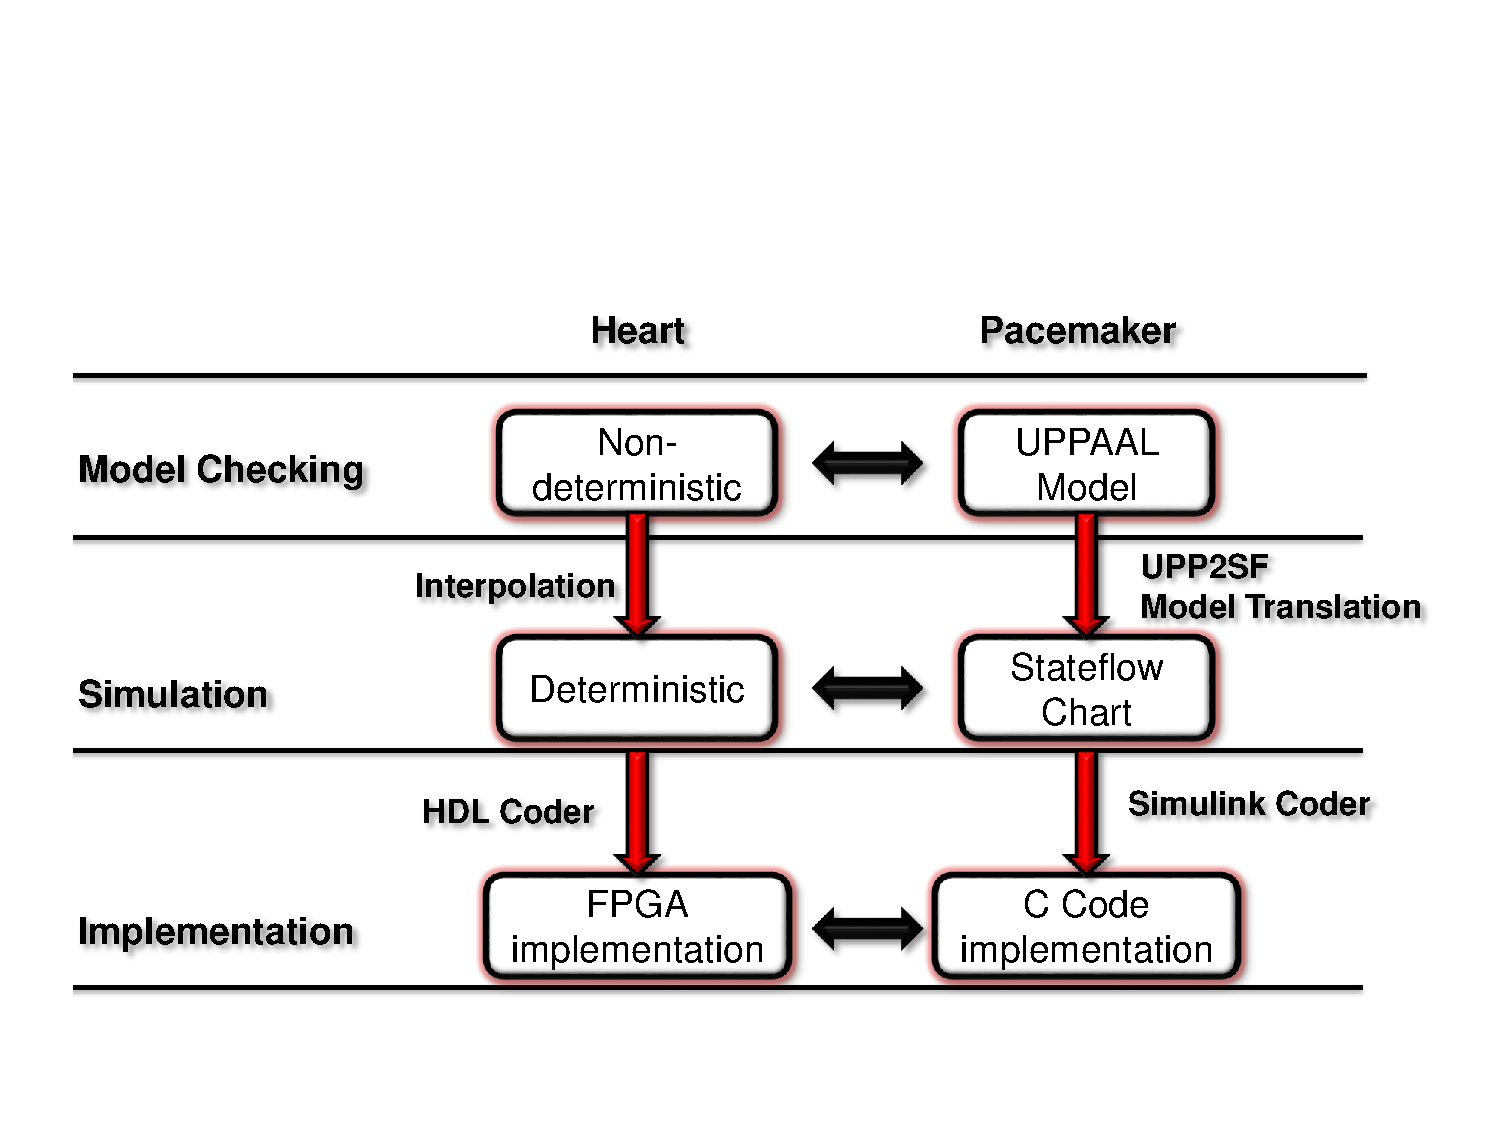
\includegraphics[scale=0.45]{figs/model_based_b.pdf}
	\caption{\small Model-based design of pacemaker software.}
	\label{fig:MBD}
\end{figure}
\section{Research Completed}
In this thesis, I propose a model-based design framework for closed-loop validation of closed-loop medical devices, and use implantable cardiac devices as case study.
Fig. \ref{fig:MBD} demonstrates our model-based design framework for implantable pacemaker software.
The thesis can be broken down into 4 themes:
%\subsection*{Theme 1: Physiological Modeling for Closed-loop Device Validation}
%Model-based closed-loop evaluation of medical devices require models of the physiological conditions of the patient(s) that can interact with the device model in closed-loop. 
%In this theme I focus on the following questions:
%\begin{itemize}
%\item How to model the physiology of the heart and how the heart models interact with the devices?
%\end{itemize}
%A heart model structure is developed which can be used to simulate electrical activities of the heart for various heart conditions.
%The model structure is capable of generating synthetic signals that can be used as inputs to implantable cardiac devices, and also able to respond to device outputs. 
%\begin{itemize}
%\item How good are the heart models?
%\end{itemize}
%The model structure was validated by the physicians for capable of generating physiological-relevant signals for variety of heart conditions.
%\begin{itemize}
%\item Are the heart models the same in different model-based applications?
%\end{itemize}
%Variations of the heart model structure are tuned for different applications during the software development process. 
%The heart model is also available on hardware platform to interact with an actual device in closed-loop.
%
%%The first step in the model-based design framework is risk analysis on abstract model of the device using closed-loop model checking technique.
%\subsection*{Theme 2: Implantable Cardiac Devices Modeling and Implementation}
%If the device software is developed as a model in the beginning, the traceability from the model to the implementation is crucial. 
%In this theme I focus on the following questions:
%\begin{itemize}
%\item What formalism shall the device model use?
%\end{itemize}
%In this thesis I model implantable cardiac device functions using timed-automata formalism, which is compatible with model checker UPPAAL.
%\begin{itemize}
%\item How to guarantee the traceability between the device model and the device implementation?
%\end{itemize}
%I developed a model translation tool to translate UPPAAL timed-automata models to Simulink Stateflow charts.
%The Stateflow charts can then be generated into code implementation using Simulink Coder.
%The model translation tool ensures that safety requirements validated at model level are preserved in the implementation.
%\subsection*{Theme 3: Medical Devices Risk Analysis with Closed-loop Model Checking}
%Risk analysis is an activity mandated by the regulators to ensure the safety and efficacy of the devices.
%In this theme, I focus on the following questions:
%\begin{itemize}
%\item How to do risk analysis of the device at model level?
%\end{itemize}
%Risk analysis can be performed on abstract model of the device using closed-loop model checking.
%An abstract model of the device, and heart models representing different heart conditions are modeled with timed-automata formalism in model checker UPPAAL.
%Risks of the devices are specified as properties and the closed-loop model is verified for the existence of safety violations.
%\begin{itemize}
%\item What are the requirements for the physiological models?
%\end{itemize}
%The physiological models used for closed-loop model checking should be able to cover all the physiological behaviors specified in the properties and their states should be expressive enough to maintain physiological context.
%\begin{itemize}
%\item How to balance the coverage and expressiveness of the physiological models?
%\end{itemize}
%I developed an abstraction tree structure to organize abstractions of the physiological model, which can also provide the physicians evidences returned by the model checker with physiological context(s).
%\subsection*{Theme 4: Model-based Clinical Trials}
%Model-based techniques can not only assist device development, but also capable of assisting the certification process.
%Before the devices are tested on real patients in clinical trials, \emph{model-based clinical trials (MBCT)} can be performed to increase the chance of a success trial and reduce cost in time and money.
%In this theme I use implantable cardioverter defibrillator (ICD) as example to demonstrate the use of MBCT can help planning an actual clinical trial.
%I focus on the following questions:
%\begin{itemize}
%\item How to represent the patient population in MBCT?
%\end{itemize}
%The validity of each heart model in the virtual patient population is guaranteed by the validated heart model structure developed before.
%The virtual patient population is generated by tuning the heart model parameters within the constraints of different heart conditions specified in the literature.
%\begin{itemize}
%\item How can MBCT benefit a real clinical trial?
%\end{itemize}
%The result of a real clinical trial is only useful when the number of patients required in the trial is accurately estimated.
%
%\begin{itemize}
%\item What are the other benefits of MBCT?
%\end{itemize}
%MBCT is much more flexible than an actual clinical trials, i.e. in MBCT the same virtual patient can interact with devices with different parameter settings.
%These benefits enable MBCT to provide comprehensive insights which can be very helpful in understanding the safety and efficacy of the device.
%
%%Another contribution of this thesis is to use heart models to represent virtual patient groups and perform  that can help the planning of an actual clinical trial. 
%%In this thesis, model-based clinical trials are performed to compare the performance of two implantable cardioverter defibrillators (ICD). 
%%The result of the MBCTs demonstrates comprehensive insights that match the result of the actual clinical trial, which would 
%
%The contributions above incorporate model-based design seamlessly into the existing regulation framework, and can be used to develop safer and cheaper closed-loop medical devices. 
%In this thesis, I propose a model-based design framework for closed-loop medical devices and use implantable cardiac devices as example.

%The rest of the section elaborates on the 4 themes, and the next section I will propose the additional research for my thesis.
%\newpage
\subsection{Theme 1: Physiological Modeling for Closed-loop Device Validation}
\begin{figure}[t]
	\centering
	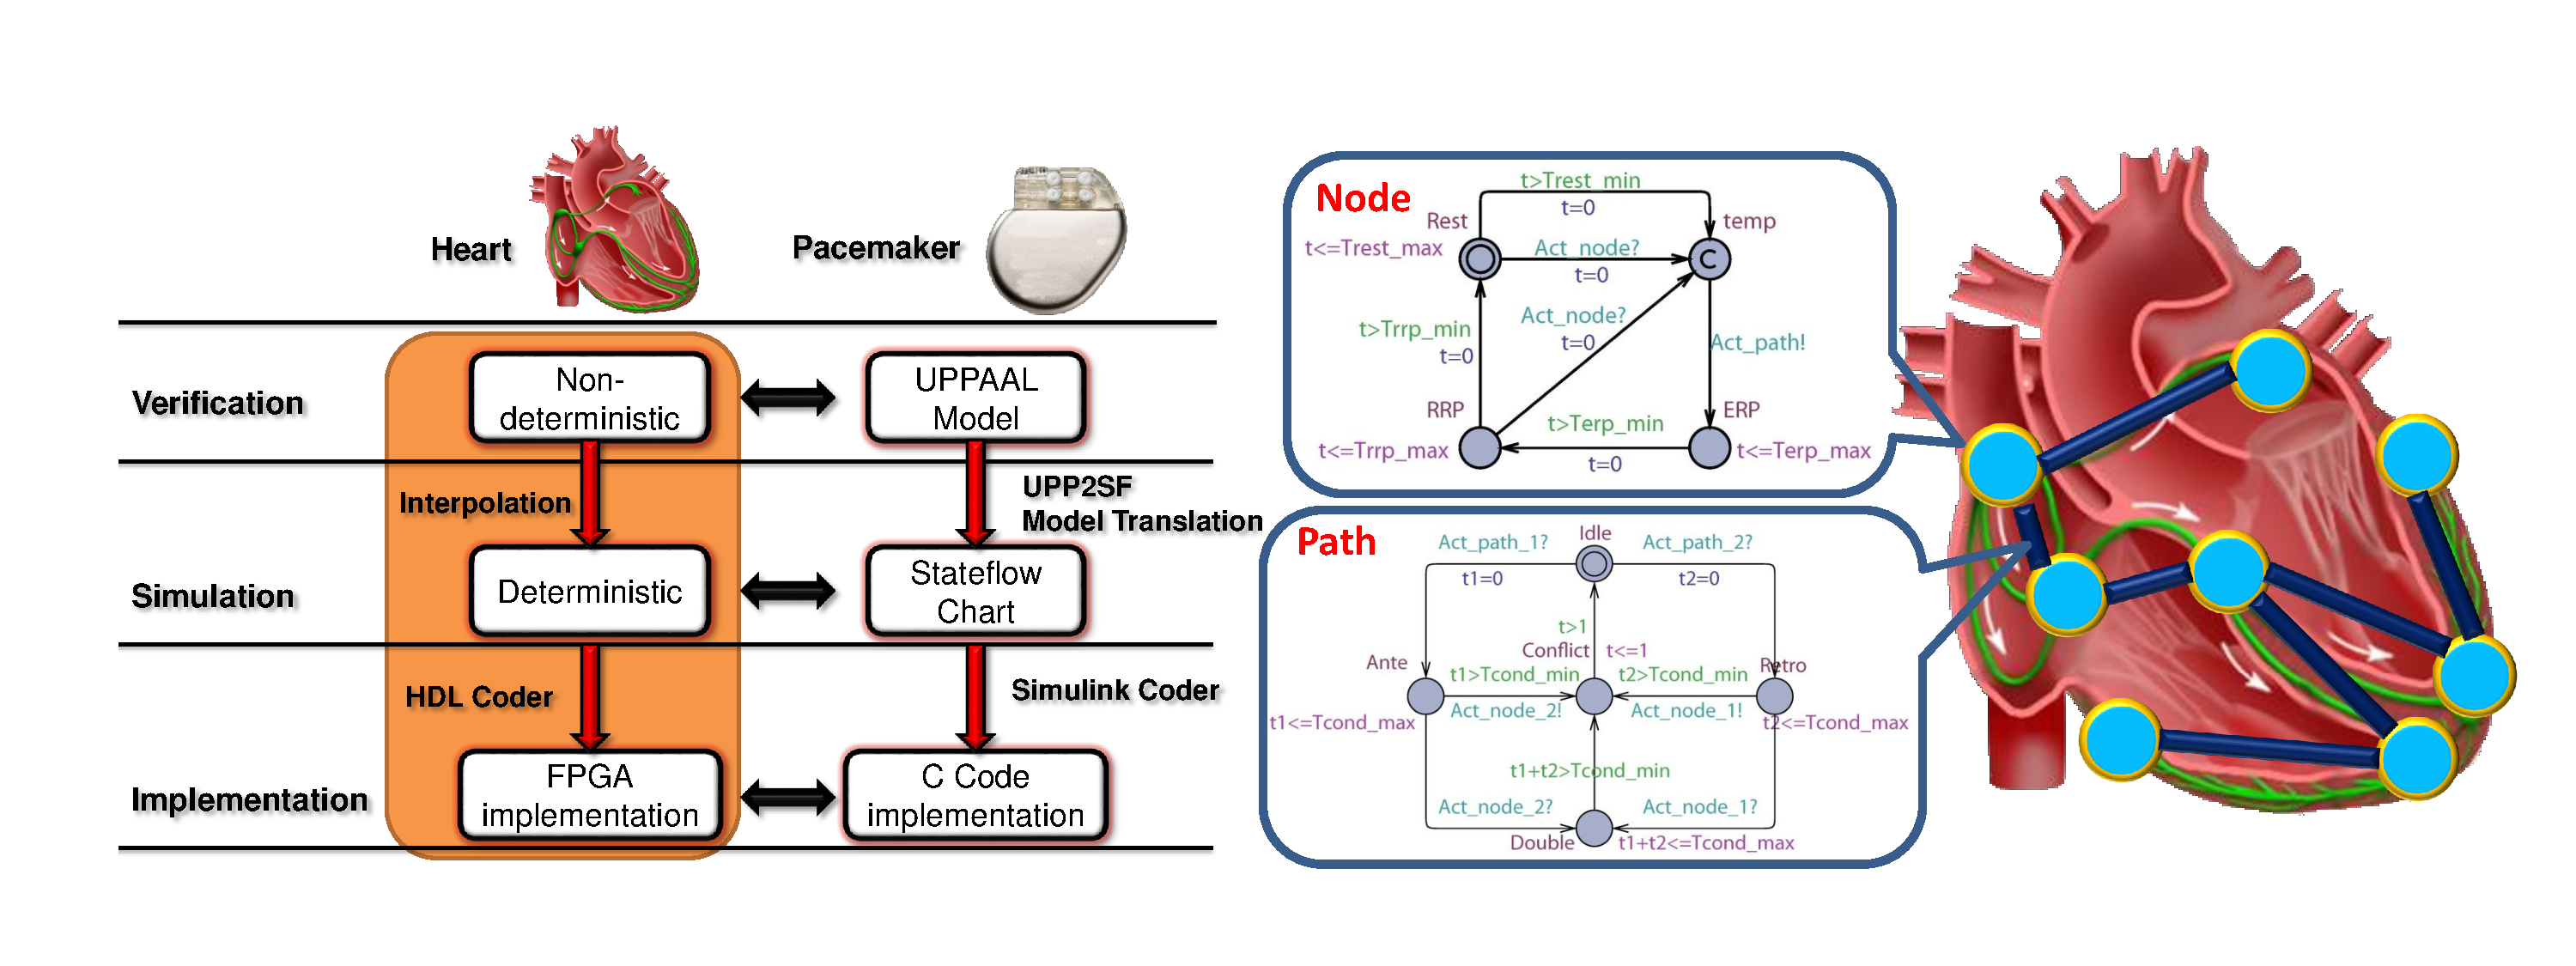
\includegraphics[scale=0.32]{figs/mb_heart.pdf}
	\caption{\small Model-based design of pacemaker software.}
	\label{fig:mb_heart}
\end{figure}
To enable closed-loop validation of the device throughout the development process, physiological models of the heart are developed to interact with the pacemaker model in closed-loop. 
In this thesis, I developed a heart model structure based on clinical electro-phisiology, which is also the foundation for implantable cardiac devices.
The heart models are capable of interacting with implantable cardiac devices in a closed-loop manner, and are available in different complexity with multiple formalisms to account for different requirements through out the design process.
\subsubsection{Electro-Physiology Model of the Heart}
The coordinated contractions of heart muscles are governed by electrical activities.
Anomalies in the timing and patterns of the electrical generation and conduction are referred to as \emph{arrhythmia}, which are the disease implantable cardiac devices are designed to treat.
I used \emph{node automata} to model the timing for electrical signal generation and blocking in heart tissue (Fig. \ref{fig:mb_heart}).
Conduction delays between node automata are modeled using \emph{path automata}.
By configuring the node and path automata with different parameters using different topology, the heart model structure can be used to model the electrical behaviors of a large varieties of heart conditions. 
The heart models can also generate realistic electrogram signals that can be used as inputs to implantable cardiac devices.

\subsubsection{Model Variations for Different Applications}
Performing closed-loop validation during different stages of the development process pose different requirements to the heart models.

During closed-loop simulation or hardware testing, the heart models should be able to capture the complex dynamics of \emph{specific hearts} to provide repeatable deterministic executions.
Therefore the heart models used for closed-loop simulation are deterministic, and include calculations for parameter changes during state transitions.

During closed-loop model checking, the heart models should be abstract enough to cover the heart behaviors of a large group of patients to account for the large variety of physiological conditions, while at the same time expressive enough to distinguish the heart behaviors specified in the property with the rest.
There is no single heart model that can satisfy both requirements, therefore a rigorous framework to balance the abstraction and refinement of the heart models is needed to select the most appropriate heart model for the physiological properties.


\subsubsection{Heart On a Chip Platform}
In order to interact with implementations of implantable cardiac devices, the heart model structure is also available on hardware. 
In this thesis, I developed the Heart On a Chip platform (Fig. \ref{fig:HOC}) which can interact with commercial pacemakers.
The heart model is implemented on a FPGA board, which interacts with the pacemaker via an analog interface.
The platform enables us to do closed-loop testing on commercially available devices, which is an important requirement if we would like to do model-based clinical trials before an actual clinical trials.
%Using the pacemaker as an example of closed-loop device, and the heart as the organ to be modeled, we present several of the challenges and early results in model-based verification.
\begin{figure}[t]
	\centering
	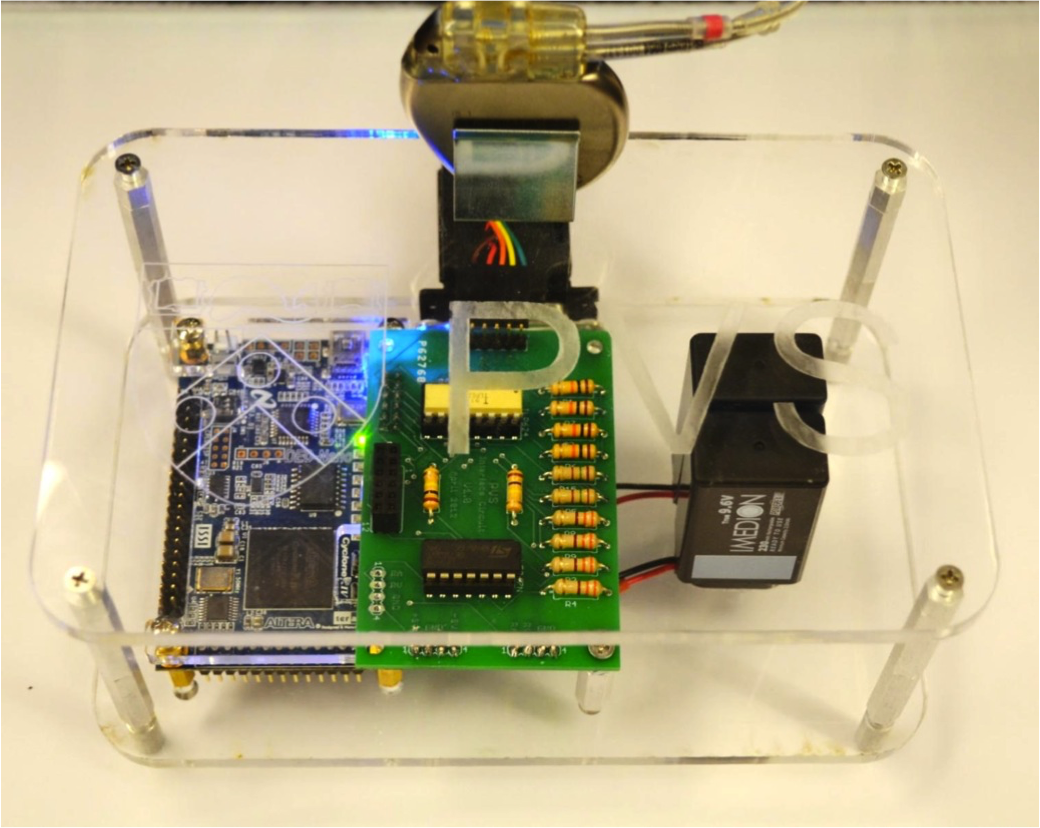
\includegraphics[scale=0.55]{figs/HOC.png}
	\caption{\small Heart On a Chip platform}
	\label{fig:HOC}
\end{figure}
\subsubsection{Heart Model Validation}
The heart model structure has been validated by demonstrating the capability to model the mechanism of different heart conditions and interact with implantable cardiac devices with generated EGM signals.
\subsubsection{Publications} 
\begin{itemize}
\item \textbf{Z. Jiang}, M. Pajic, A. Connolly, S. Dixit, and R. Mangharam. Real-time heart model
for implantable cardiac device validation and verification. In Real-Time Systems
(ECRTS), 2010 22nd Euromicro Conference on, pages 239 –248, July 2010.
\item \textbf{Z. Jiang}, M. Pajic, and R. Mangharam. Cyber-Physical Modeling of Implantable
Cardiac Medical Devices. Proceedings of the IEEE, 100(1):122 –137, Jan. 2012a.
\item \textbf{Z. Jiang}, M. Pajic, R. Alur, and R. Mangharam. Closed-loop verification of medical
devices with model abstraction and refinement. International Journal on Software
Tools for Technology Transfer, 16(2):191–213, 2014.
\item \textbf{Z. Jiang} and R. Mangharam. Modeling Cardiac Pacemaker Malfunctions with the
Virtual Heart Model. In Engineering in Medicine and Biology Society,EMBC,
2011 Annual International Conference of the IEEE, pages 263 –266, Sept 2011.
\item \textbf{Z. Jiang}, M. Pajic, and R. Mangharam. Model-based Closed-loop Testing of Implantable Pacemakers. In ACM/IEEE Second International Conference on Cyber-
Physical Systems (ICCP’11), 2011.
\end{itemize}



\newpage
\subsection{Theme 2: Medical Devices Risk Analysis with Closed-loop Model Checking}
\begin{figure}[t]
	\centering
	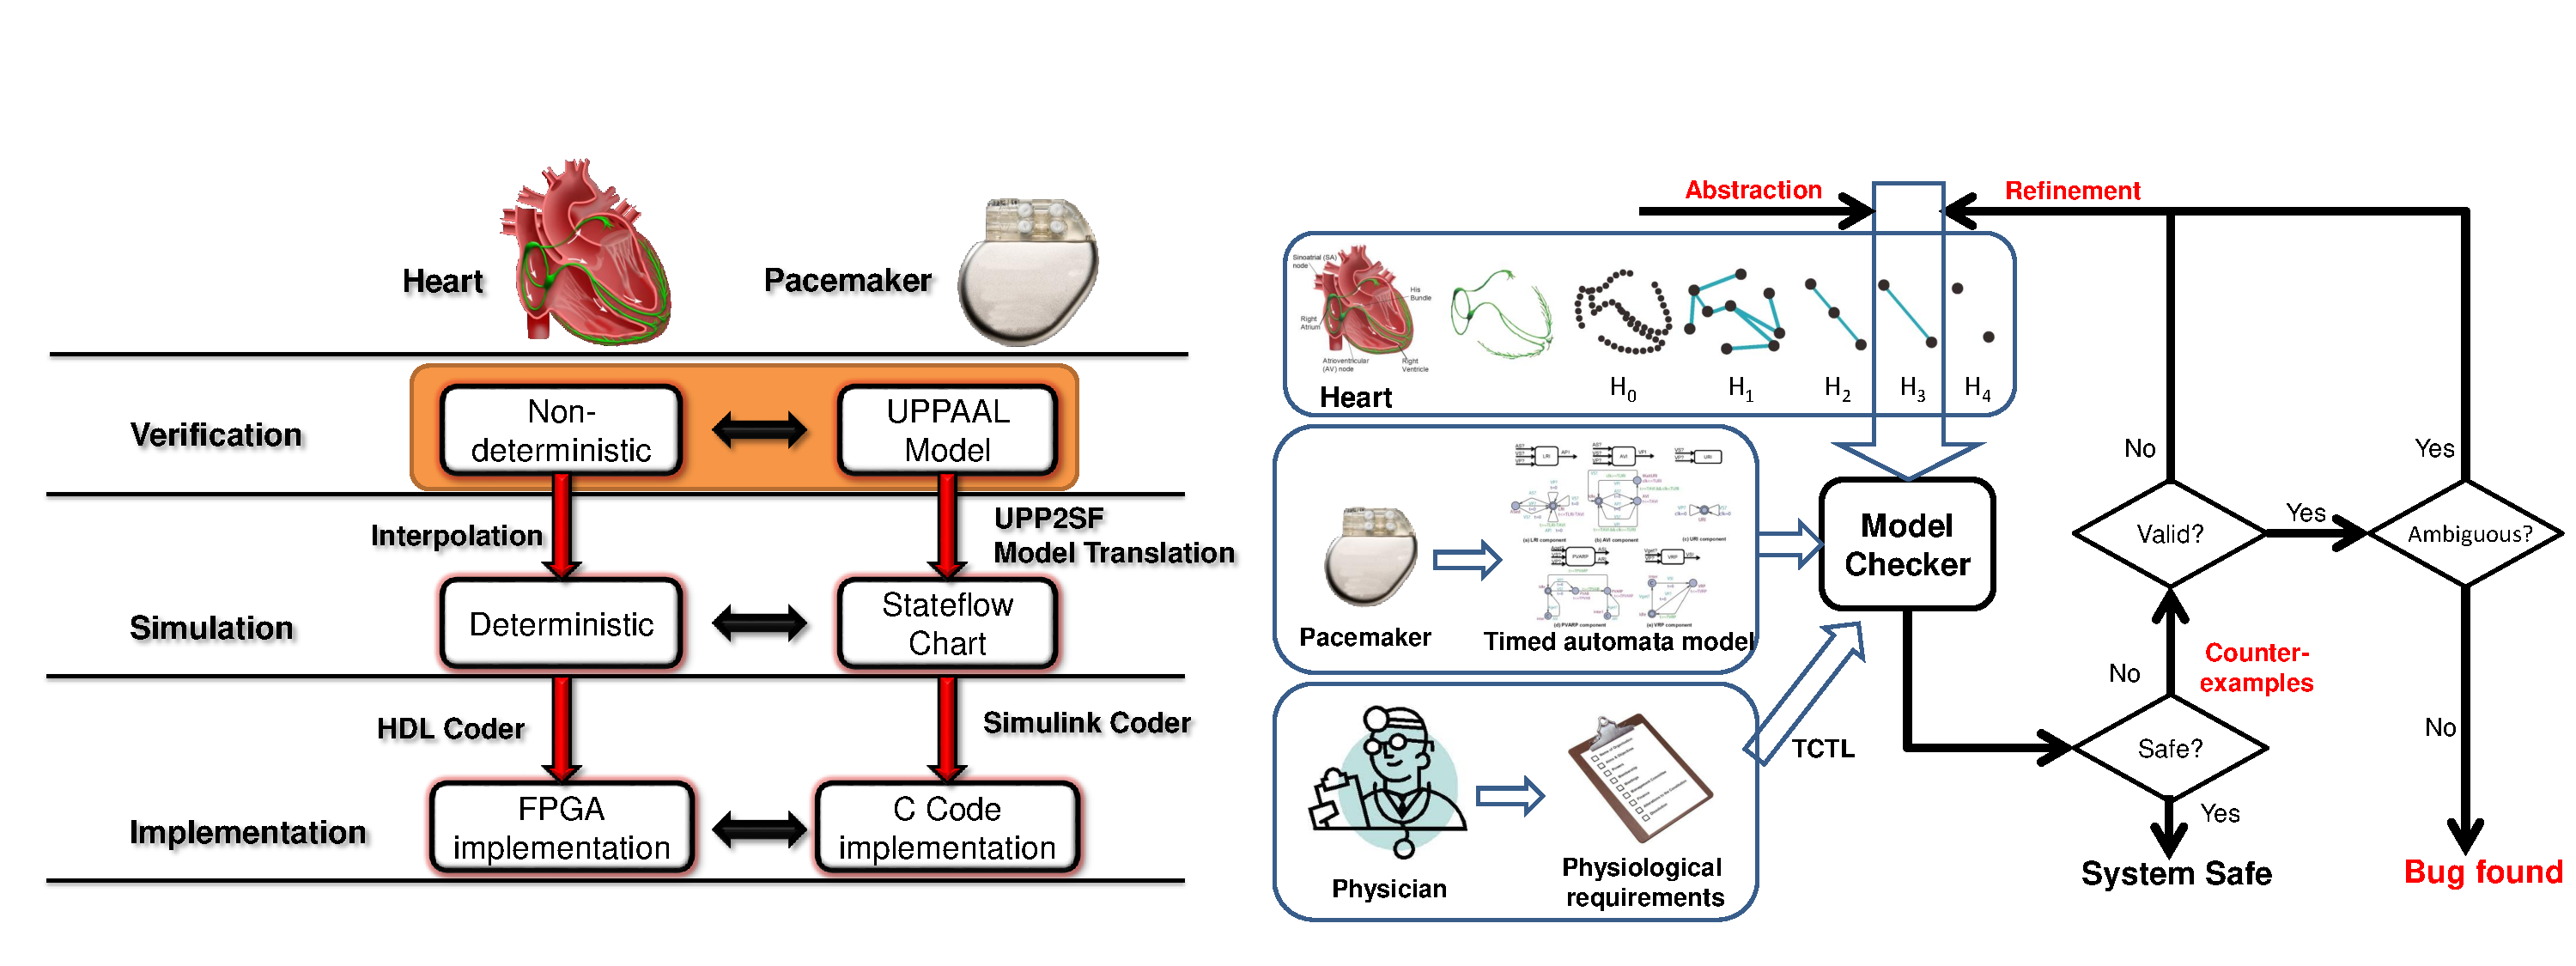
\includegraphics[scale=0.32]{figs/mb_mc.pdf}
	\caption{\small Model-based design of pacemaker software.}
	\label{fig:mb_mc}
\end{figure}
Risk analysis is an activities mandated by the regulator to provide confidence to the safety of the device, which is currently done manually.
Model checking has been widely used in semi-conductor industry which can check the whole state space of a model for property violations.
However, model checking has not been applied in the medical device industry due to the lack of appropriate physiological models.
In this thesis the heart model structure has been modified to non-deterministically cover electrical behaviors of a large number of heart conditions.
A rigorous abstraction and refinement framework has been developed to choose the most appropriate heart model for a physiological property.
In the thesis, I did risk analysis on a dual chamber implantable pacemaker, which includes risks that can endanger the safety of the patients.
By specifying these risks as physiological properties, I used model checking to identify safety violations of the abstract pacemaker model.
This research demonstrates the potential for application of model checking in the medical device industry.

\subsubsection{Risk Analysis for Implantable Pacemaker}
In this thesis, I focused on two most intuitive risks that an implantable pacemaker can pose on patients: 1) The pacemaker fails to increase the ventricular rate no lower than 60bpm, and 2) The ventricular rate is increased inappropriately by the pacemaker.
Fault Tree Analysis (FTA) has been performed on the two risks to identify known and unknown causes for the two risks. 
Fig. \ref{fig:FTA} demonstrates the FTA for a car and one of the risks for pacemaker.
\subsubsection{Closed-loop Model Checking for Risk Analysis of Implantable Pacemaker}
All identified causes for the two risks have been specified as TCTL properties.
The closed-loop model which consists of the device model and a physiological model are then verified in model checker UPPAAL.
UPPAAL returns evidences of these risks as execution traces, if any.
In this thesis, we were able to identify evidences for risks in our pacemaker model, which are almost impossible to find with traditional testing methods.
For the additional algorithms designed to terminate Pacemaker Mediated Tachycardia, which is one of the risks, we evaluated their performance in terms of whether the risks have been reasonably \emph{mitigated}.

With tools like quantitative model checker, we can also evaluate the frequency and severity of the remaining risks, which is an important part in risk analysis.
All of the analysis above can be used as evidence for the safety of the device model.
\begin{figure}[t]
	\centering
	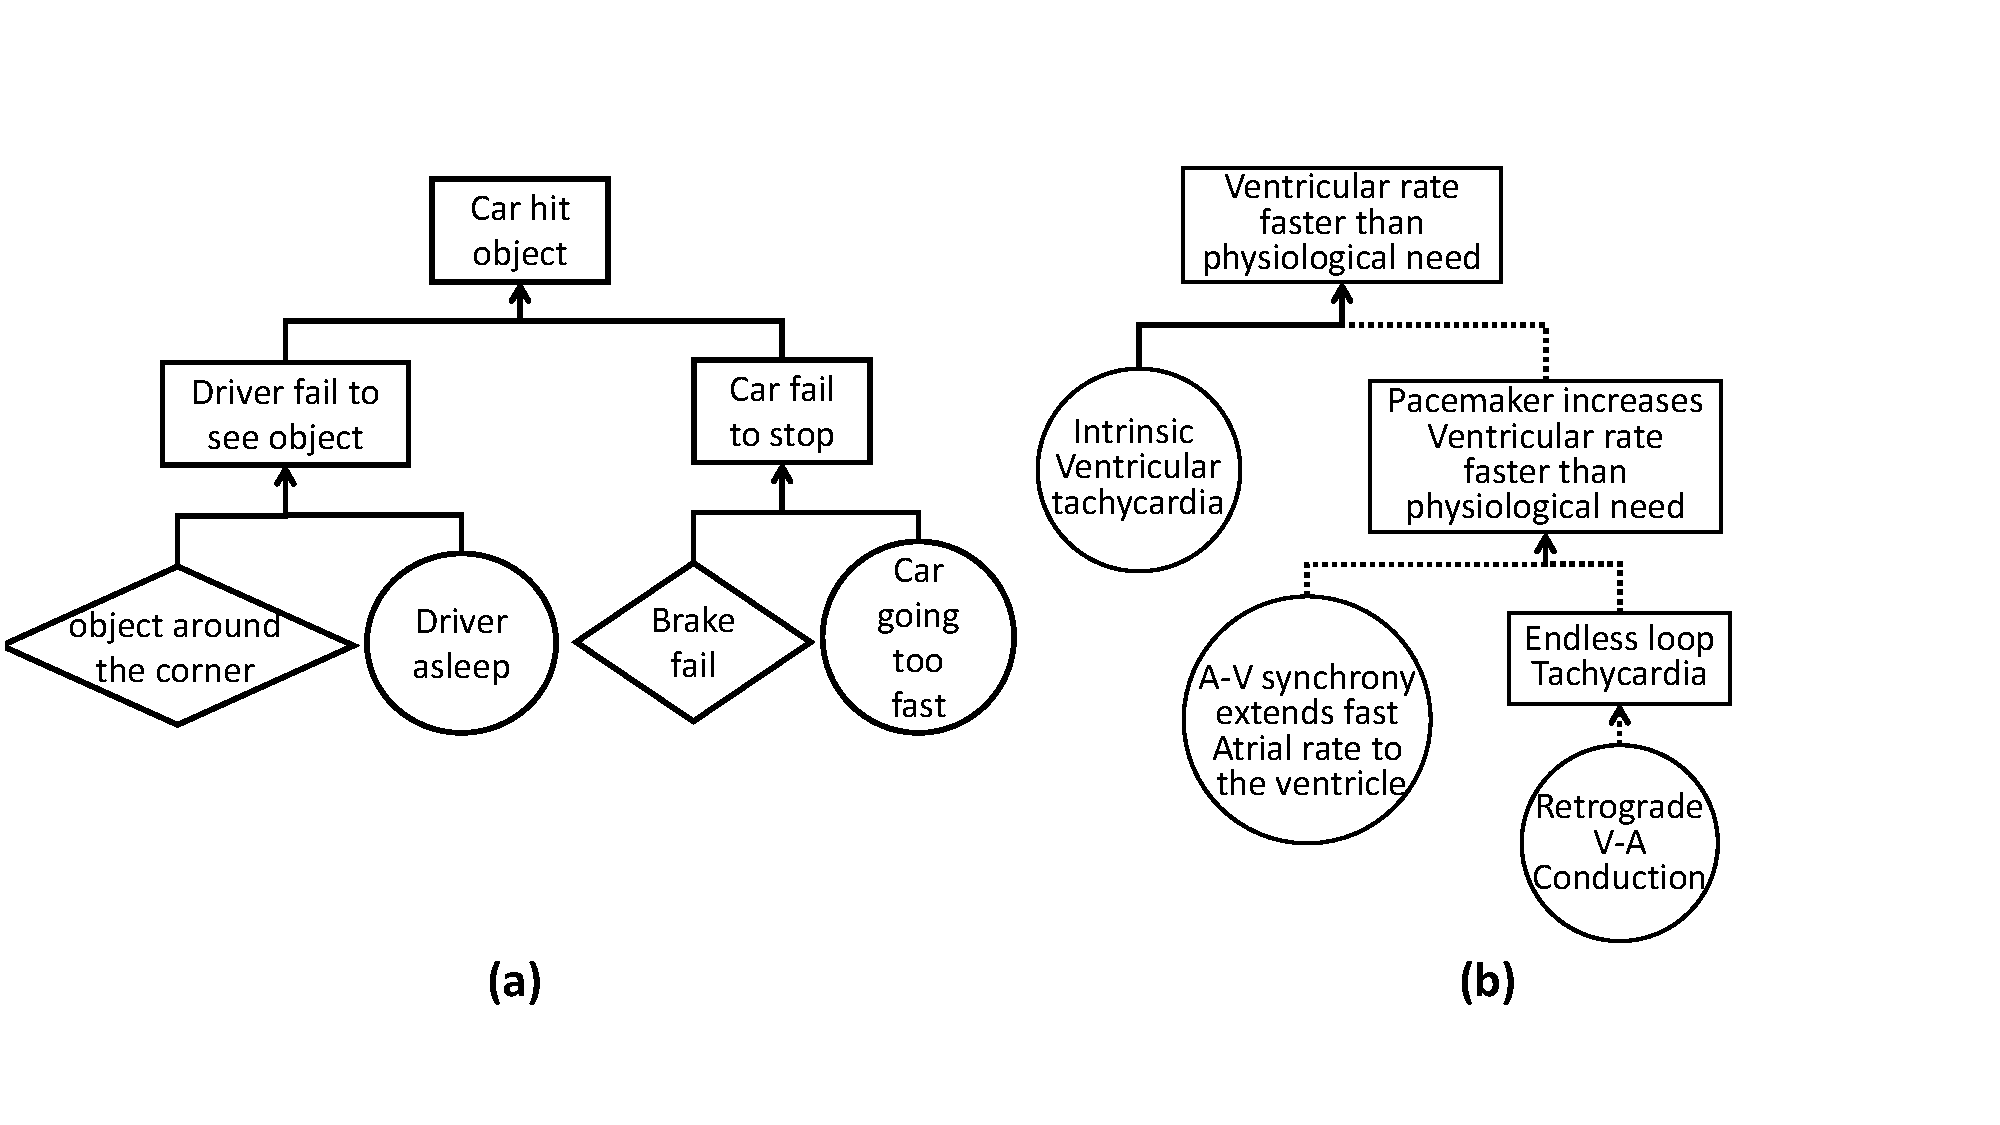
\includegraphics[scale=0.35]{figs/FTA_new.pdf}
	\caption{\small Fault Tree Analysis}
	\label{fig:FTA}
\end{figure}
\subsubsection{Heart Model Abstraction and Refinement}

The major challenge for closed-loop model checking is to develop appropriate physiological models. 
The models should be general enough to cover physiological behaviors from different patient conditions, while at the same time expressive enough to maintain physiological meanings of an execution trace.
There is no single model that can satisfy both requirements for different properties.
Using models that are too abstract introduces false-negatives, while using models too specific introduces false-positives.
Moreover, with multiple physiological models, their relationships in terms of coverage is difficult to know, which reduces the rigorousness of the results.
It is therefore important to have a rigorous hierarchy of physiological models with different abstraction levels and a procedure to choose the appropriate model for a property.

In this thesis, we adopted the Counter-Example-Guided Abstraction and Refinement framework to balance the coverage and expressiveness of the heart models (Fig. \ref{fig:mb_mc}).
Each property is checked with the heart model with the most behavior coverage.
If an evidence is returned by the model checker, it is manually analyzed for its physiological validity.
If the evidence is valid, it is then checked for ambiguity due to the over-abstraction of the model. 
If the evidence is both valid and unambiguous, the execution is a true evidence for the risk property.
\subsubsection{Abstraction Tree for Physiological Model Abstraction and Refinement (in progress)}
The method above requires enormous amount of domain knowledge and is time consuming.
Therefore we are proposing an automated and rigorous framework for physiological modeling during closed-loop model checking.

First, a set of initial heart models are created by the physicians to cover behaviors of possible heart conditions.
The initial set is by no mean exhaustive but provides a solid foundation for model abstraction.
Then by applying physiological abstraction rules, the heart models and their behaviors are merged into more abstract models.
The abstraction rules introduce new behaviors into the more abstract model which are mostly physiological relevant.
By applying physiological abstraction rules in certain order we obtain a tree-like structure for heart model abstractions, which we refer to as the \emph{Abstraction Tree}.
During model checking, the most abstract model which covers all possible behaviors of the heart is first used to interact with the device.
If a counter-example is found, it is then analyzed in more refined heart models following the abstraction tree for both validity check and de-ambiguity.
In the end, the counter-example is either valid in one or more concrete heart models, which provides physiological contexts to the counter-example; or only valid in an intermediate abstraction level, which will be checked by the physician for validity.

The abstraction tree effectively separates the physiological domain and the computer science domain, which encourages the application of model checking in medical device development and certification.
\subsubsection{Publications}
\begin{itemize}
\item \textbf{Z. Jiang}, M. Pajic, S. Moarref, R. Alur, and R. Mangharam. Modeling and Verification
of a Dual Chamber Implantable Pacemaker. Tools and Algorithms for the
Construction and Analysis of Systems, 7214:188–203, 2012b.
\item \textbf{Z. Jiang}, M. Pajic, R. Alur, and R. Mangharam. Closed-loop verification of medical
devices with model abstraction and refinement. International Journal on Software
Tools for Technology Transfer, 16(2):191–213, 2014.
\end{itemize}

\newpage

\subsection{Theme 3: Implantable Cardiac Devices Modeling and Implementation}
\begin{figure}[t]
	\centering
	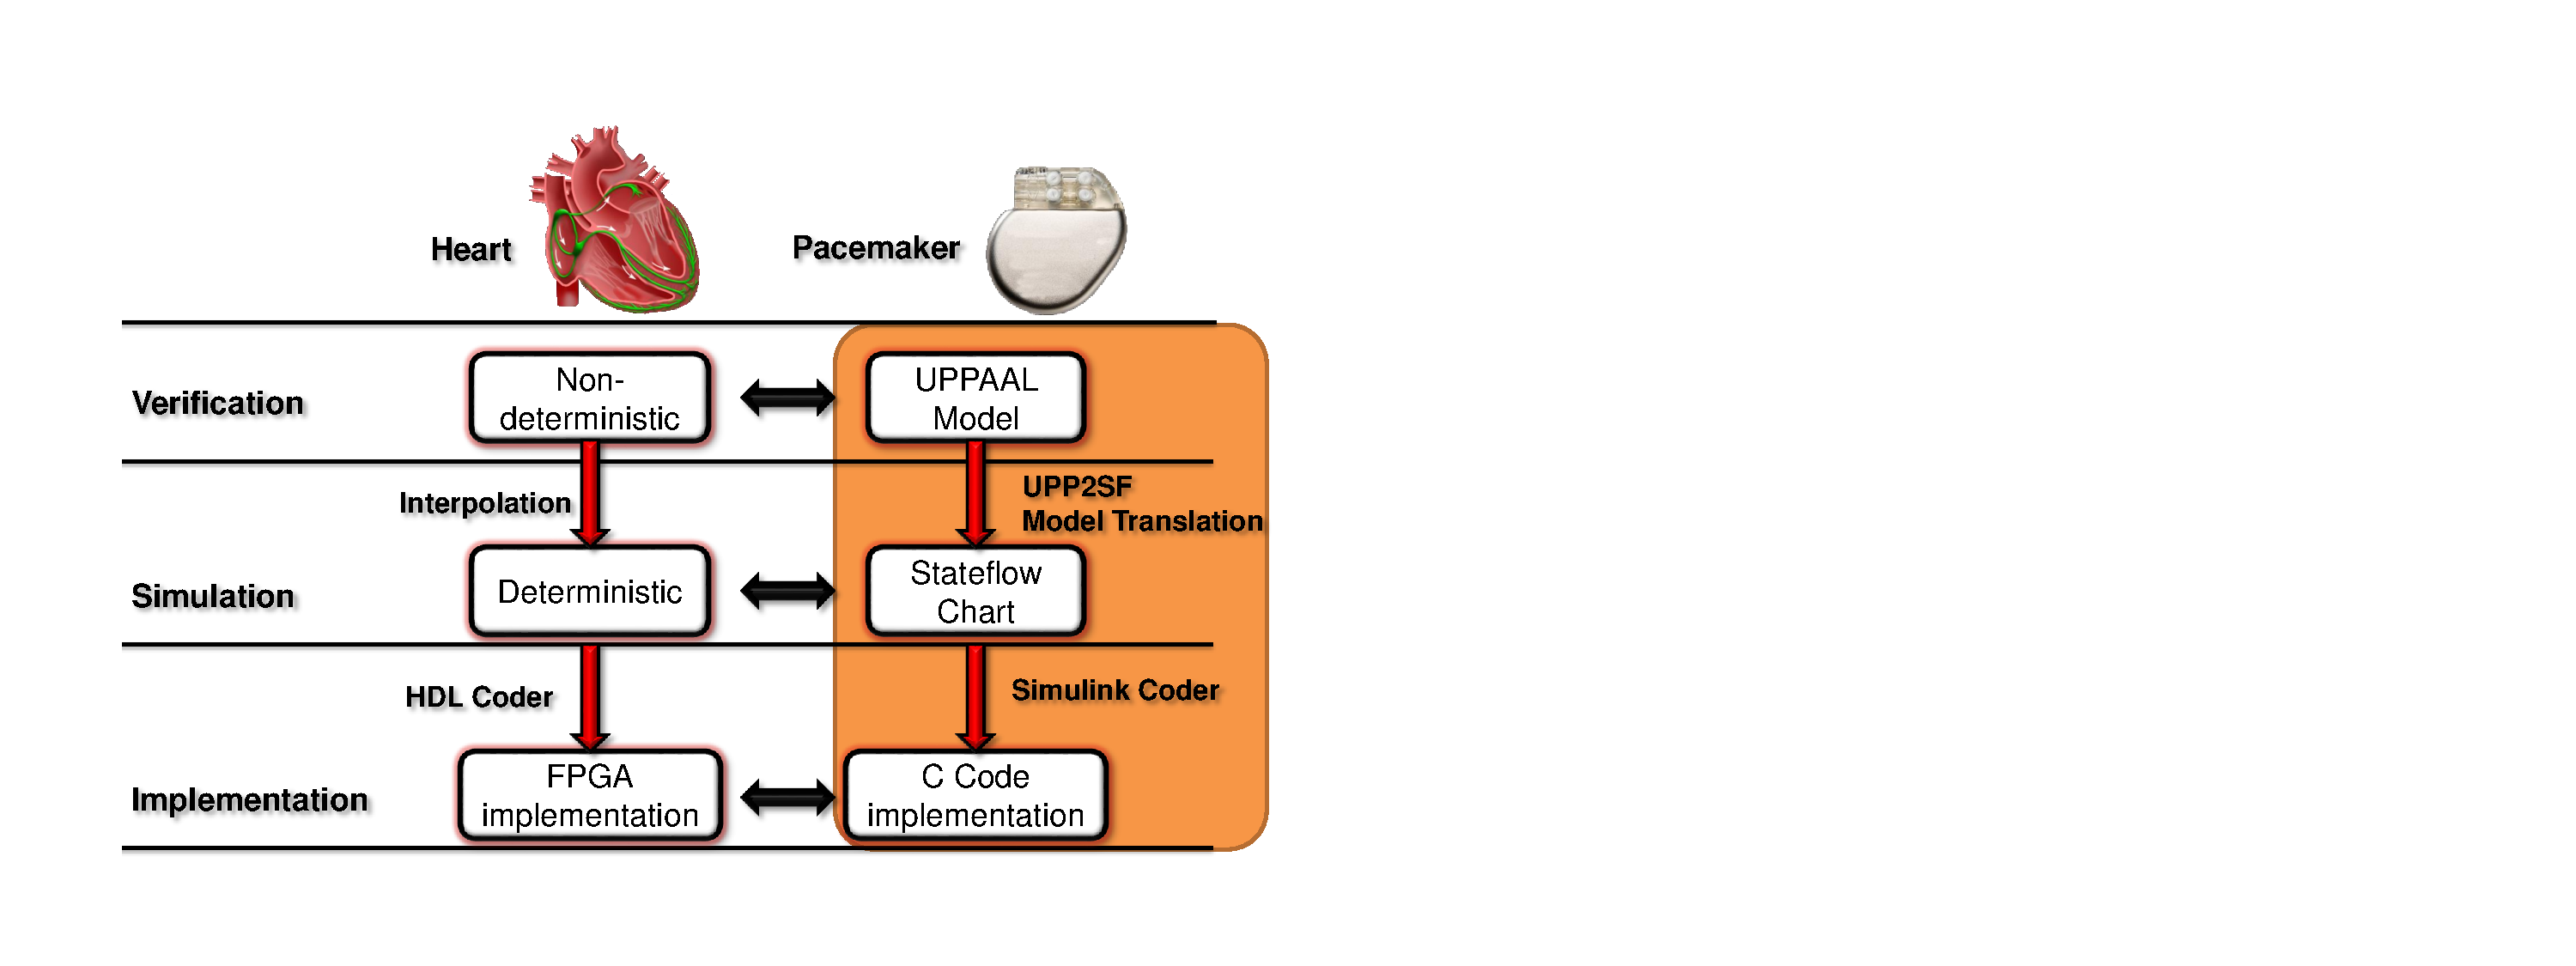
\includegraphics[scale=0.32]{figs/mb_device.pdf}
	\caption{\small Model-based design of pacemaker software.}
	\label{fig:mb_device}
\end{figure}
In this thesis I tried to demonstrate model-based development process for implantable cardiac devices.
Therefore models of the device functions at different design stage are essential to enable white-box evaluation of the device functions.
It is also important to ensure \emph{traceability} between models of the devices and device implementations.
In this thesis I implemented models for implantable pacemaker and developed model translation tool chain to generate device implementations automatically and rigorously.
\subsubsection{UPPAAL Model of a Dual Chamber Pacemaker}
A dual chamber pacemaker senses local electrical events from the right atrium and right ventricle, respectively.
The software diagnoses the heart condition by comparing the timing relationship among events.
Electrical pacing will be delivered to restore normal heart rhythm if the heart rate is low.
Therefore it is intuitive to model the pacemaker functionality as timed-automata.
In this thesis, I modeled a dual chamber pacemaker as timed-automata in model checker UPPAAL, using specifications from publicly-available literature (Fig. \ref{fig:mb_device}).
The model includes the basic 5 timing cycles of a dual chamber pacemaker.
I also implemented two additional algorithms that were designed to eliminate \emph{Pacemaker Mediated Tachycardia (PMT)}, during which the pacemaker inappropriately increase the heart rate.
Through the experiment I validated the performance of the PMT algorithms, and also evaluated whether implementing additional functionality can violate properties satisfied by the original model.
\subsubsection{UPP2SF Model Translation}
Due to the limited semantics of the model checking tool, the device model in the model checker is generally an abstraction of the actual device functions.
The biggest challenge for model implementation tool chain is how to deal with the additional behaviors in the actual implementation, and how they affect the property preservation.
After the device model has mitigated all the risks, it is essential for the device implementation to preserve those properties.
In our framework, we developed a model translation tool which rigorously translates device model in UPPAAL model checker to Stateflow chart.
The Stateflow chart can then be compiled into C code implementation using Simulink Coder, which completes a tool chain from validated model to validated code.

\subsubsection{Publications}
\begin{itemize}
\item \textbf{Z. Jiang}, M. Pajic, S. Moarref, R. Alur, and R. Mangharam. Modeling and Verification
of a Dual Chamber Implantable Pacemaker. Tools and Algorithms for the
Construction and Analysis of Systems, 7214:188–203, 2012b.
\item M. Pajic, \textbf{Z. Jiang}, I. Lee, O. Sokolsky, and R. Mangharam. From Verification to
Implementation: A Model Translation Tool and a Pacemaker Case Study. In Proceedings
of the 2012 IEEE 18th Real Time and Embedded Technology and Applications
Symposium, RTAS ’12, pages 173–184, 2012.
\item M. Pajic, \textbf{Z. Jiang}, I. Lee, O. Sokolsky, and R. Mangharam. Safety-critical medical
device development using the upp2sf model translation tool. ACM Trans. Embed.
Comput. Syst., 13(4s):127:1–127:26, 2014.
\end{itemize}

\newpage

\begin{figure}[t]
	\centering
	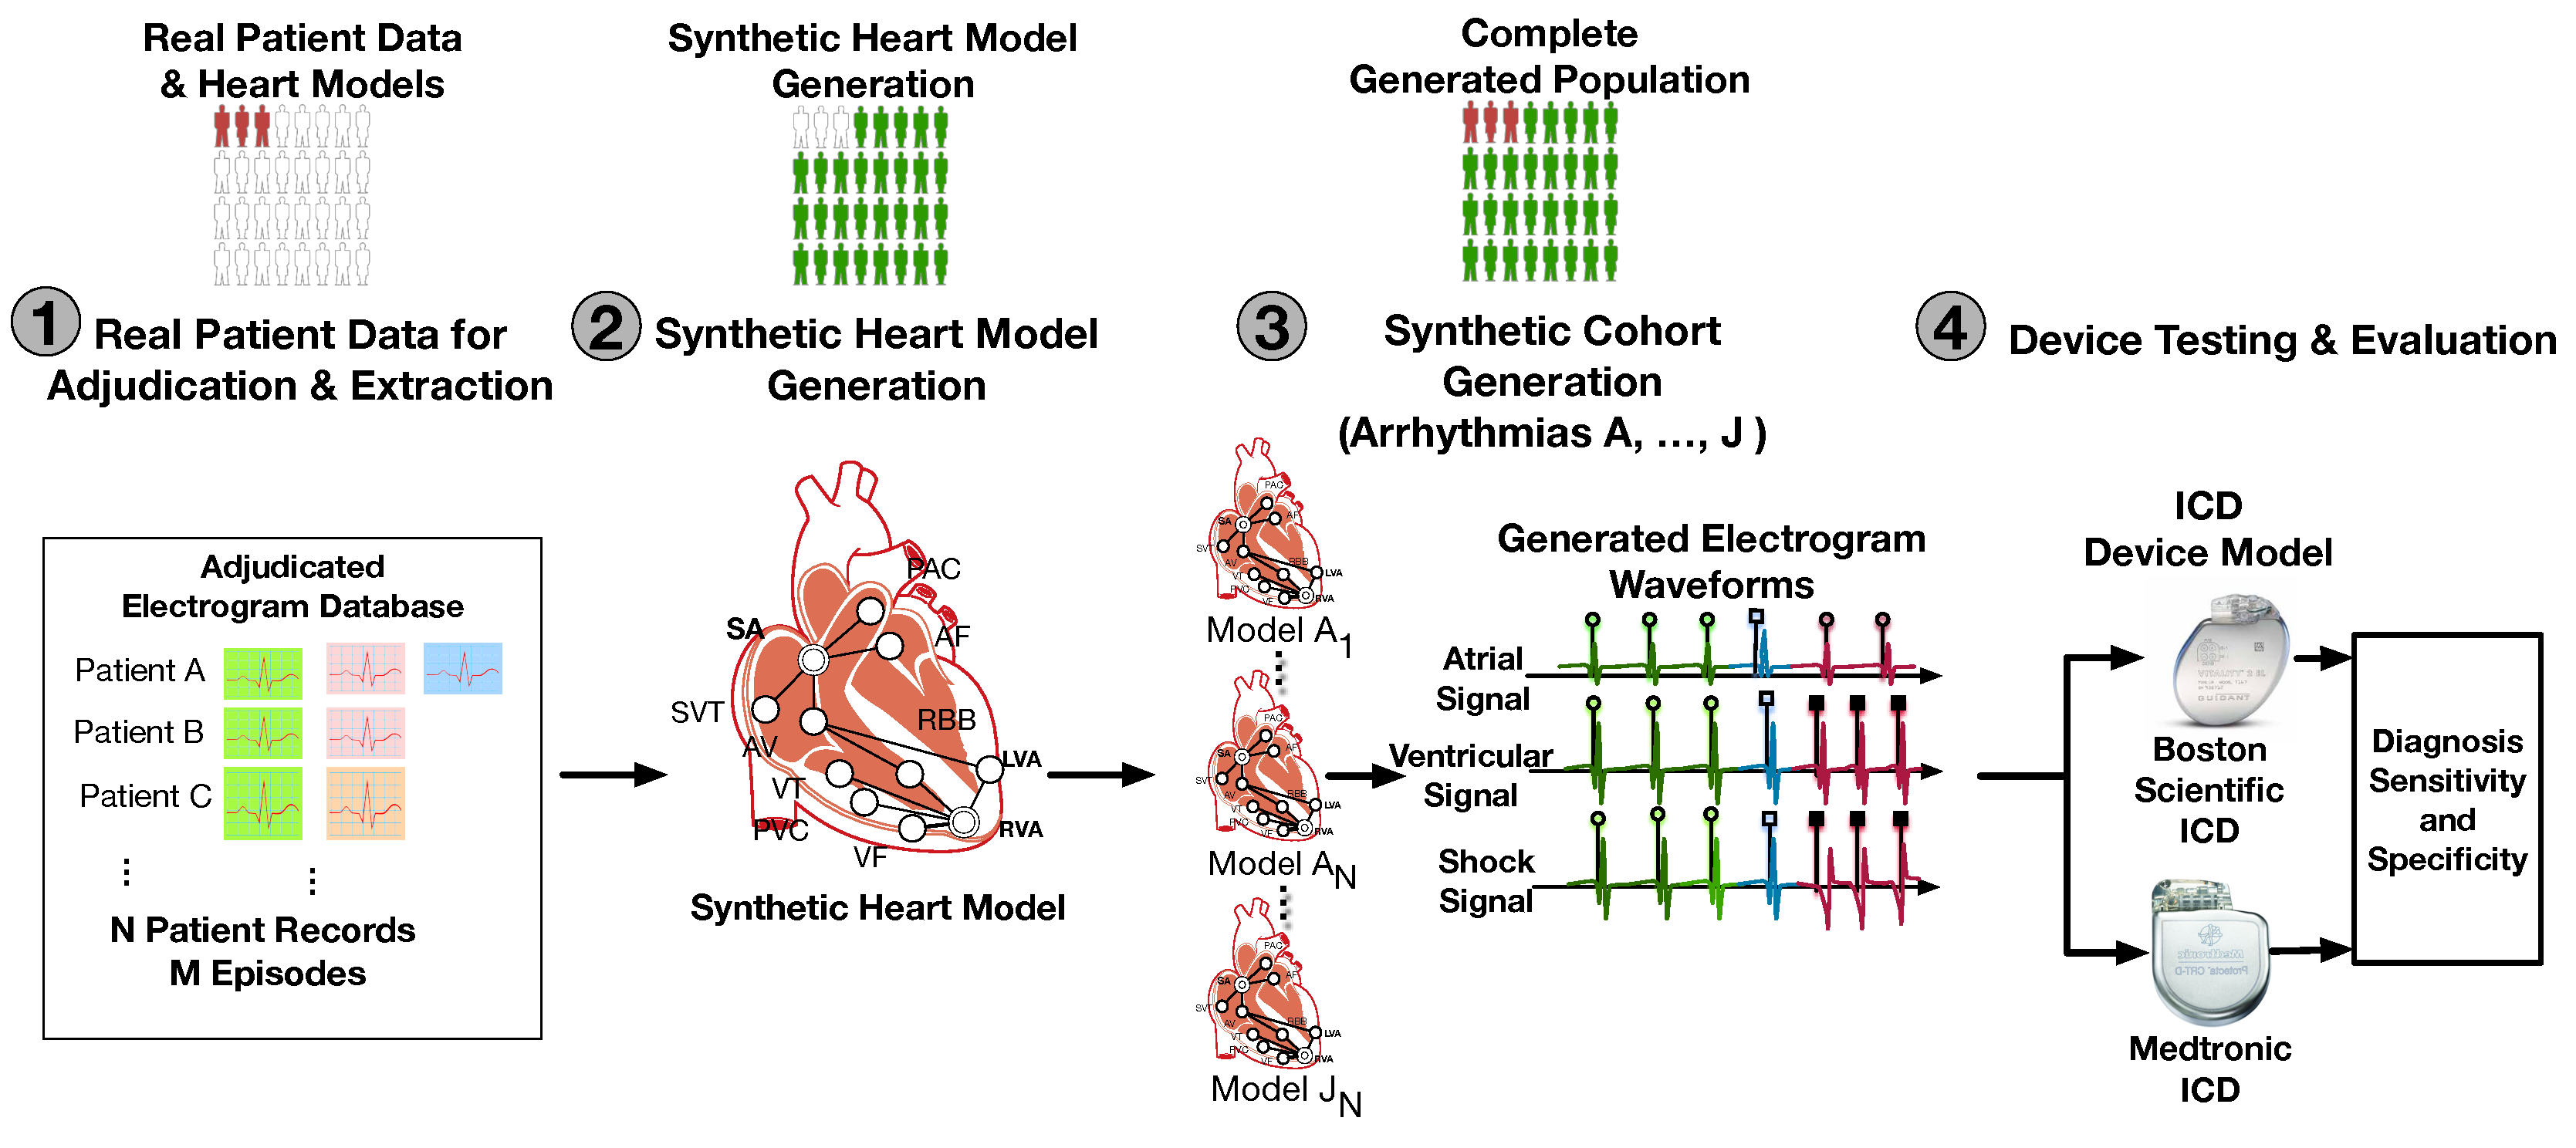
\includegraphics[scale=0.25]{figs/figMBCToverview.pdf}
	\caption{\small Model-based Clinical Trials for Implantable Cardiac Devices}
	\label{fig:mbct}
\end{figure}
\subsection{Theme 4: Model-based Clinical Trials for Medical Devices (in progress)}
%Due to the limitations of the formalism used during model checking, there are aspects that cannot be captured by the abstract models at the model checking stage.
%Therefore closed-loop testing is a necessary complement for model checking to identify potential safety issue originated from aspects that were abstracted away during model checking. 
%In this thesis, I established a closed-loop testing framework for implantable cardiac devices, with deterministic heart models interacting with device models in closed-loop.
%%The heart models in Stateflow can be configured into different heart conditions
Clinical trials is the ultimate validation for a medical device before the device can be released to the market.
Clinical trials for medical devices are costly in terms of both time and money, therefore they should be carefully planned to reduce the risk of failures.
Currently clinical trials for medical devices are planned with data from previous trials and studies, which do not reflect the current patient population and/or technology advancement.
Clinical trials planned based on these historical data have high chance of failure, which not only cost a lot of money and time, but also pose significant risks on patients involved.

In this theme, I propose \emph{Model-based Clinical Trials (MBCT)} which can be performed before the clinical trial and provide useful insights to guide the actual clinical trial.
\subsubsection{Virtual Population Generation}
The biggest question for MBCT is how comparable the model-based virtual population is to the real patient population. 
Our current approach is to learn the constraints on parameters for the parametrized model using a sample of real patients' data, as indicated by markers \circled{1} and \circled{2} in Fig. \ref{fig:mbct}. 
Ideally this sample of patients is a population from a previous trial.
These learned constraints are then used to generate more instances of the model (marker \circled{3}), and this constitutes our model cohort.

\subsubsection{Model-based RIGHT}
With generated virtual population, the device is then connected to these models (marker \circled{4}) and the outcomes of interest are evaluated.
In this work, we mimicked the RIGHT trial in which two different ICDs are compared in terms of inappropriate therapy.
The result of our MBCT shows comparable results to the actual trial, which is a validation of our virtual population.
We also used the flexibility of the MBCT to perform more analysis which cannot be performed during a real trial (i.e. evaluate devices with different parameter settings on the same patient).

An MBCT is \emph{not} a replacement for a clinical trial: rather, it will allow us to run very large-scale targeted simulated trials to better inform our conduct of an actual clinical trial.
This provides valuable insight into which patients should be enrolled in the trial (and in whom the device is most efficacious).
Another application would be to get tighter estimates of statistical quantities like effect size needed before the conduct of the trial. 
%
%\subsubsection{Physiological Requirement Hierarchy}
%Due to the limited diagnostic and therapeutic capability of closed-loop medical devices, it is impossible for the devices to restore the patient's condition to an absolutely optimal condition.
%The devices should be able to restore the patients' maximum health within its capabilities.
%However some compromises have to be made among all physiological requirements that define "healthy". 
%
%In this thesis, I listed physiological requirements that defines "healthy heart" and assigned priorities to them.
%For an open-loop heart which violates some of the requirements, the closed-loop system with the device should always attempt to satisfy requirements with higher priority.
%Monitors for each requirement are also developed in Simulink to automatically monitor the closed-loop system and report requirement violations.
%\subsubsection{Crosstalk and Lead Displacement}
%One of the aspects that are abstracted during model checking is the sensing component of the pacemaker.
%However, sensing errors correspond to a large number of device malfunctions.
%
%In this thesis, I demonstrated two most common causes for sensing error: crosstalk and lead displacement.
%Fig. \ref{fig:mb_sim} demonstrates a lead displacement case in which the atrial lead of a dual chamber pacemaker dislodged and dropped into the ventricle.
%A new artificial pathway is then established between the atrial lead and the ventricular lead, which is much shorter than the intrinsic pathway.
%The pacemaker is not aware of the dislodge and functions as usual, which may miss therapy and endanger the patient.
%The heart model is capable of modeling the mechanism of lead displacement and identify potential safety hazards.
\subsubsection{Publications}
\begin{itemize}
\item H. Abbas, \textbf{Z. Jiang}, K. Jang, Rahul Mangharam, Model-based Clinical Trials for Medical Devices. International Conference on Cyber-Physical Systems, 2016 (Submitted).
\end{itemize}

\newpage
\subsection{Publications}
\subsubsection{Conference Publications}
\begin{itemize}
\item \textbf{Z. Jiang}, M. Pajic, A. Connolly, S. Dixit, and R. Mangharam. Real-time heart model
for implantable cardiac device validation and verification. In Real-Time Systems
(ECRTS), 2010 22nd Euromicro Conference on, pages 239 –248, July 2010.
\item \textbf{Z. Jiang} and R. Mangharam. Modeling Cardiac Pacemaker Malfunctions with the
Virtual Heart Model. In Engineering in Medicine and Biology Society,EMBC,
2011 Annual International Conference of the IEEE, pages 263 –266, Sept 2011.
\item \textbf{Z. Jiang}, M. Pajic, and R. Mangharam. Model-based Closed-loop Testing of Implantable
Pacemakers. In ACM/IEEE Second International Conference on Cyber-
Physical Systems (ICCP’11), 2011.

\item \textbf{Z. Jiang}, M. Pajic, S. Moarref, R. Alur, and R. Mangharam. Modeling and Verification of a Dual Chamber Implantable Pacemaker. Tools and Algorithms for the
Construction and Analysis of Systems, 7214:188–203, 2012b.
\item M. Pajic, \textbf{Z. Jiang}, I. Lee, O. Sokolsky, and R. Mangharam. From Verification to
Implementation: A Model Translation Tool and a Pacemaker Case Study. In Proceedings
of the 2012 IEEE 18th Real Time and Embedded Technology and Applications
Symposium, RTAS ’12, pages 173–184, 2012.
\end{itemize}
\subsubsection{Journal Publications}
\begin{itemize}
\item \textbf{Z. Jiang}, M. Pajic, and R. Mangharam. Cyber-Physical Modeling of Implantable
Cardiac Medical Devices. Proceedings of the IEEE, 100(1):122 –137, Jan. 2012a.
\item \textbf{Z. Jiang}, M. Pajic, R. Alur, and R. Mangharam. Closed-loop verification of medical
devices with model abstraction and refinement. International Journal on Software
Tools for Technology Transfer, 16(2):191–213, 2014.
\item M. Pajic, \textbf{Z. Jiang}, I. Lee, O. Sokolsky, and R. Mangharam. Safety-critical medical
device development using the upp2sf model translation tool. ACM Trans. Embed.
Comput. Syst., 13(4s):127:1–127:26, 2014.
\end{itemize}
\subsubsection{Book Chapters}
\begin{itemize}
\item \textbf{Z. Jiang} and R. Mangharam. High-Confidence Medical Device Software
Development. Foundations and Trends in Electronic Design Automation, Vol. 9, No. 4 (2015) 309–391.
\end{itemize}
\subsubsection{Magazine Publication}
\begin{itemize}
\item \textbf{Z. Jiang}, H. Abbas, K. Jang and R. Mangharam. Towards high confidence medical device software. IEEE Computer Jan 2016 Outlook
\end{itemize}
\subsection{Awards}

\begin{itemize}
	\item Best Student Paper Award, 18th IEEE Real-Time and Embedded Technology and Applications Symposium (RTAS), April 2012
	\item Best Paper Award Nominee, Tools and Algorithms for the Construction and Analysis of Systems (TACAS), March 2012
	\item 1st Prize(Award of Excellence) of High-tech Medical Service, The World Embedded Software Contest (WESC), December 2012
	\item Best in Session Award, SRC TECHCON 2014, Sep 2014
\end{itemize}

\newpage

\section{Proposed Research}
The proposed research focus on improving certain steps in the model-based design framework, and proposing new methodology to the regulation of medical devices to complement the model-based design framework.
\subsection{Abstraction Tree for Physiological Modeling During Closed-loop Model Checking}
As discussed earlier, during closed-loop model checking of medical devices, there is need to abstract and refine the physiological models according to avoid introducing false-positives and false-negatives to the model checking results.
In my previous work, abstraction and refinement are performed manually which also requires extensive domain knowledge.
Moreover, physiological models lose their physiological context during abstraction, therefore evidence traces returned from an abstract model may be difficult to interpret by the domain experts, and there may be multiple concrete execution traces corresponding to the abstract trace, causing ambiguities.

In the proposed research, I would like to introduce an automated and rigorous framework which encode the domain knowledge into an abstraction tree structure, so that developer performing model checking can automatically obtain the most appropriate heart model for the property, and if an evidence trace returns, it is concretized into the most concrete physiological condition(s) for the domain experts to examine.
\begin{figure}[t]
	\centering
	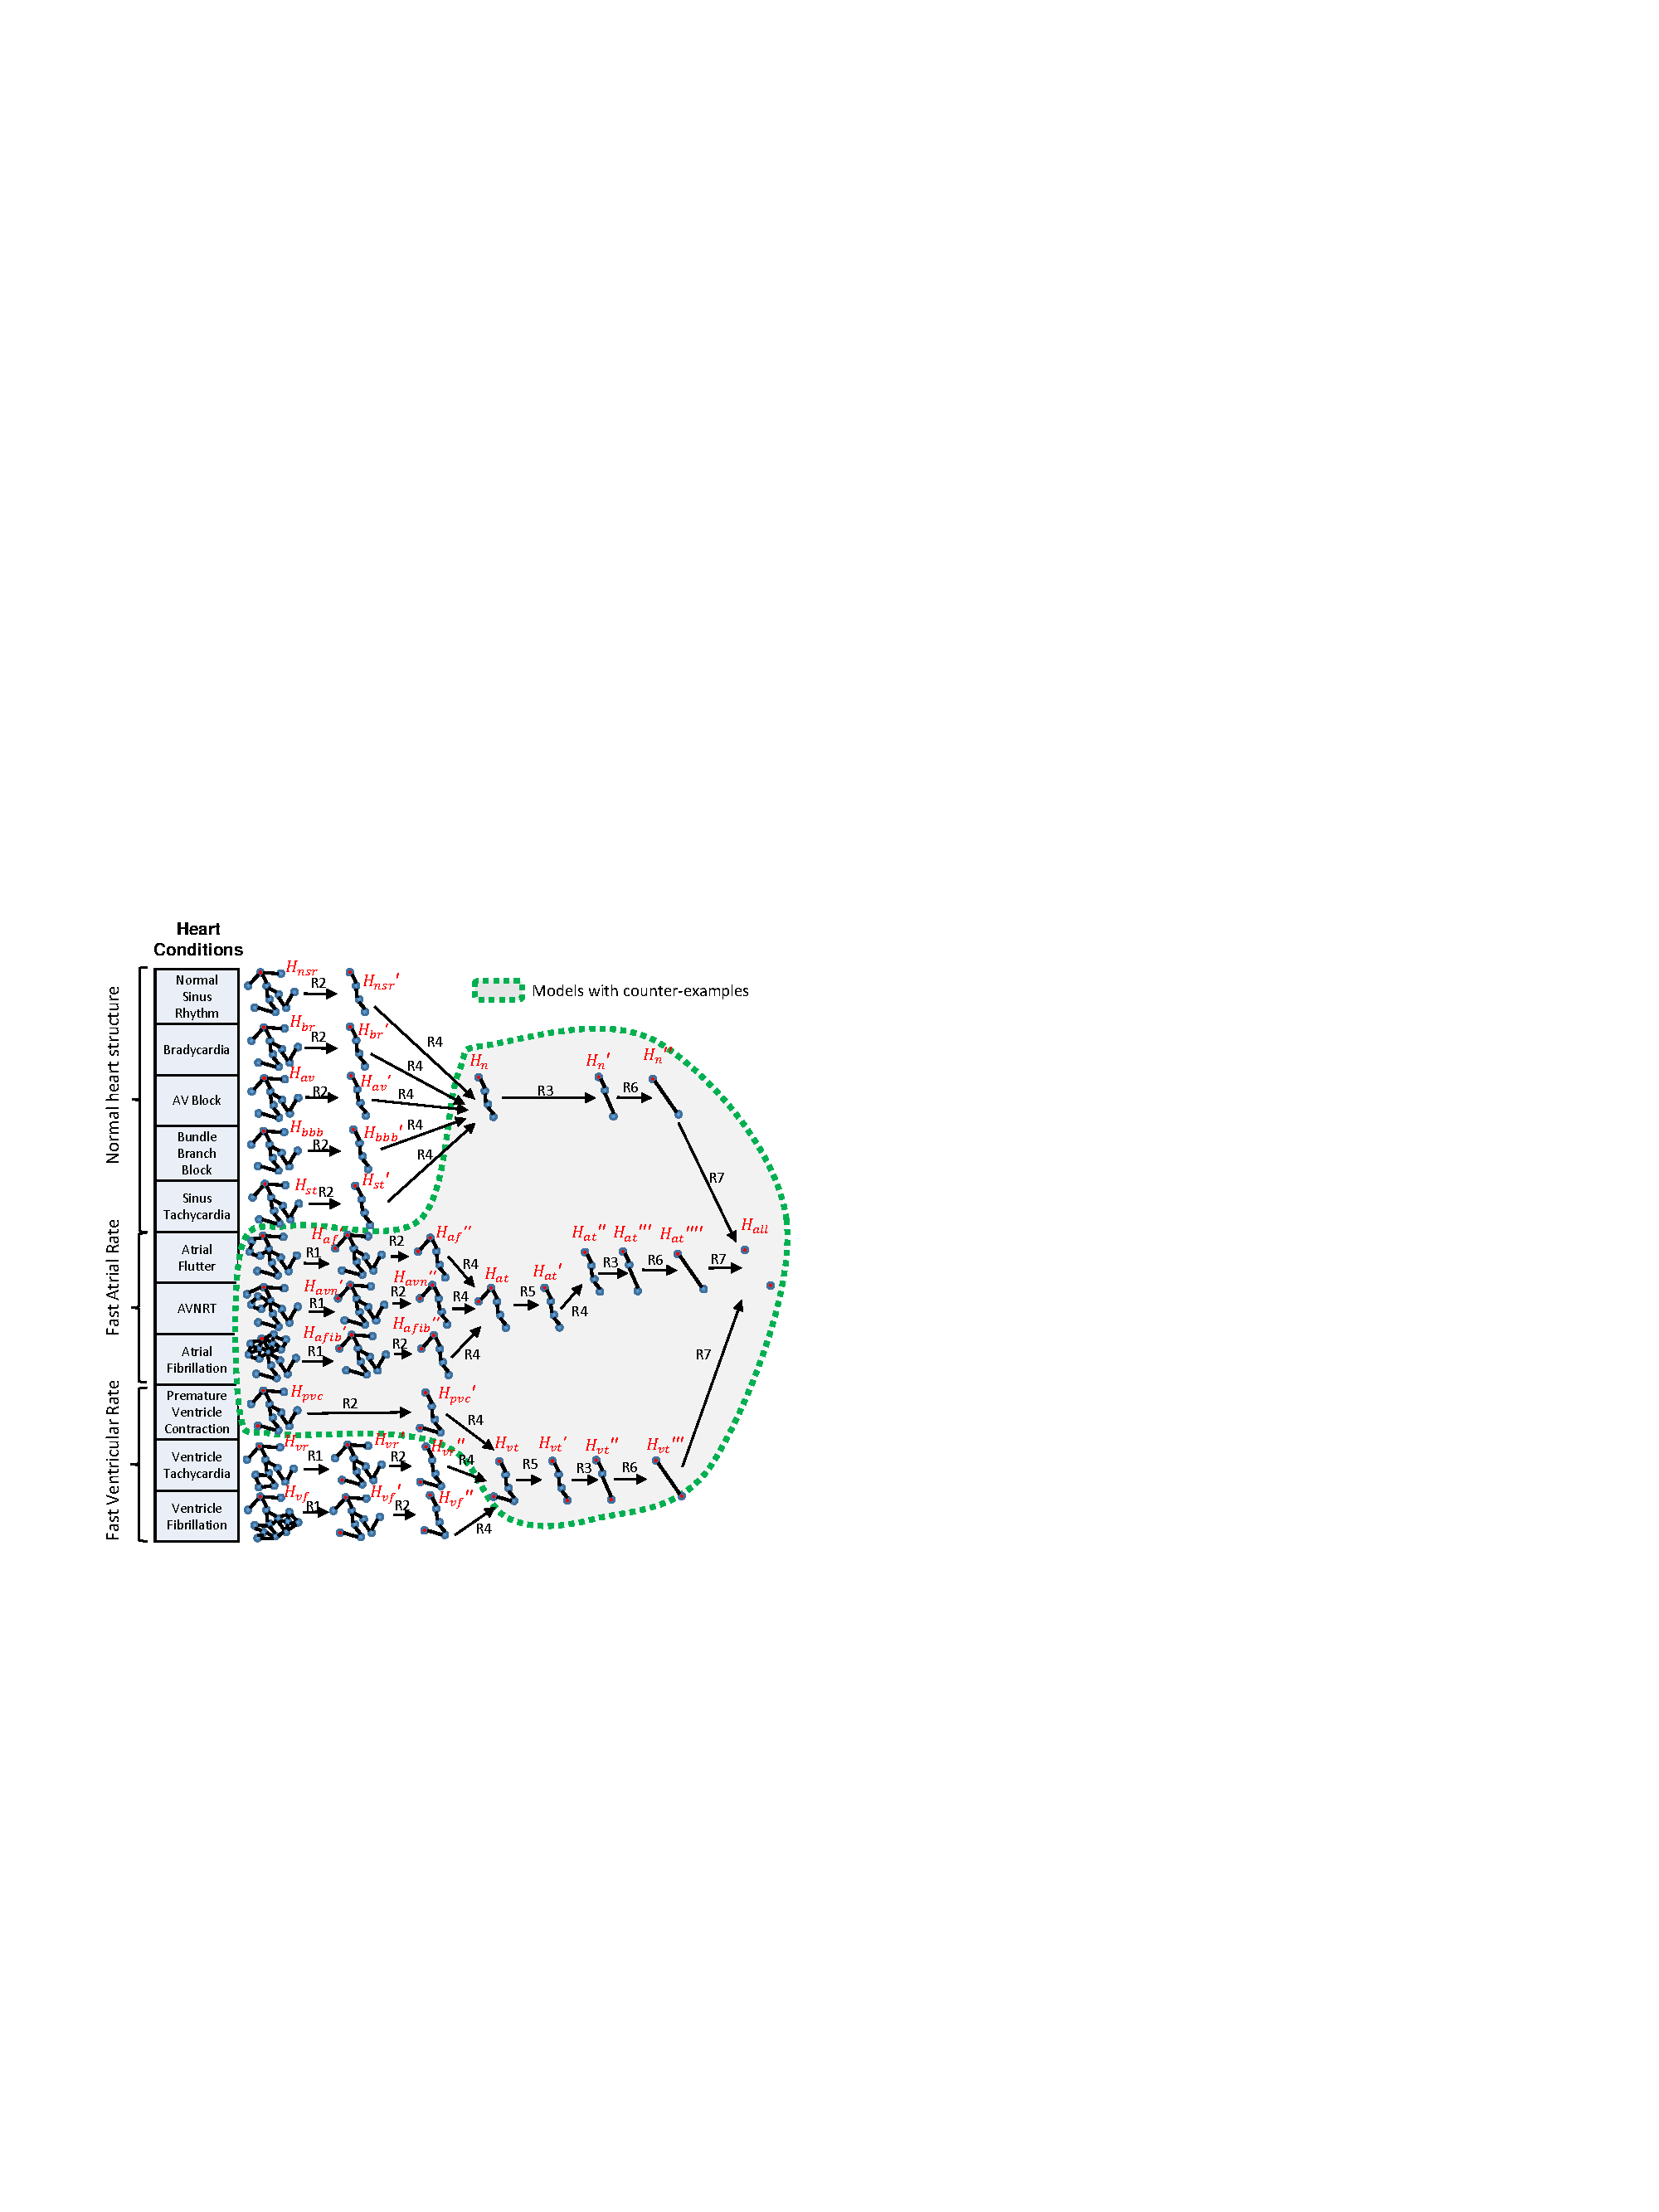
\includegraphics[scale=0.7]{figs/abs.pdf}
	\caption{\small Model-based Clinical Trials for Implantable Cardiac Devices}
	\label{fig:mbct}
\end{figure}
\subsection{Model-based Clinical Trials for Closed-loop Medical Devices}
Clinical trials is the ultimate validation for a medical device before the device can be released to the market.
Clinical trials for medical devices are costly in terms of both time and money, therefore they should be carefully planned to reduce the risk of failures.
Currently clinical trials for medical devices are planned with data from previous trials and studies, which do not reflect the current patient population and/or technology advancement.
Clinical trials planned based on these historical data have high chance of failure, which not only cost a lot of money and time, but also pose significant risks on patients involved.

In this thesis, I propose \emph{Model-based Clinical Trials (MBCT)}, which use physiological models to generate a virtual patient population.
By running a trials on the virtual population, we can gain useful insights that can be helpful when planning an actual clinical trials.
The validity of MBCT results relies heavily on the validity of the physiological model and the validity of the virtual patient population, which is the biggest challenge for MBCT.
MBCT is not designed to replace clinical trials.
But performing MBCT before the clinical trials provides more confidence to the safety and efficacy of the devices, and can potentially reduce the chance of trial failures.
%\subsubsection{ICD models}
\end{document}